\documentclass[notes,11pt, aspectratio=169]{beamer}

\usepackage{pgfpages}
% These slides also contain speaker notes. You can print just the slides,
% just the notes, or both, depending on the setting below. Comment out the want
% you want.
\setbeameroption{hide notes} % Only slide
%\setbeameroption{show only notes} % Only notes
%\setbeameroption{show notes on second screen=right} % Both

\usepackage{helvet}
\usepackage[default]{lato}
\usepackage{array}
\usepackage{tgbonum}

\usepackage{tikz}
\usepackage{verbatim}
\setbeamertemplate{note page}{\pagecolor{yellow!5}\insertnote}
\usetikzlibrary{positioning}
\usetikzlibrary{snakes}
\usetikzlibrary{calc}
\usetikzlibrary{arrows}
\usetikzlibrary{decorations.markings}
\usetikzlibrary{shapes.misc}
\usetikzlibrary{matrix,shapes,arrows,fit,tikzmark}
\usepackage{amsmath}
\usepackage{mathpazo}
\usepackage{hyperref}
\usepackage{lipsum}
\usepackage{multimedia}
\usepackage{graphicx}
\usepackage{multirow}
\usepackage{graphicx}
\usepackage{dcolumn}
\usepackage{bbm}
\newcolumntype{d}[0]{D{.}{.}{5}}

\usepackage{changepage}
\usepackage{appendixnumberbeamer}
\newcommand{\beginbackup}{
   \newcounter{framenumbervorappendix}
   \setcounter{framenumbervorappendix}{\value{framenumber}}
   \setbeamertemplate{footline}
   {
     \leavevmode%
     \hline
     box{%
       \begin{beamercolorbox}[wd=\paperwidth,ht=2.25ex,dp=1ex,right]{footlinecolor}%
%         \insertframenumber  \hspace*{2ex} 
       \end{beamercolorbox}}%
     \vskip0pt%
   }
 }
\newcommand{\backupend}{
   \addtocounter{framenumbervorappendix}{-\value{framenumber}}
   \addtocounter{framenumber}{\value{framenumbervorappendix}} 
}


\usepackage{graphicx}
\usepackage[space]{grffile}
\usepackage{booktabs}
\newcommand\independent{\protect\mathpalette{\protect\independenT}{\perp}}
\def\independenT#1#2{\mathrel{\rlap{$#1#2$}\mkern2mu{#1#2}}}
\DeclareMathOperator{\Supp}{Supp}

% These are my colors -- there are many like them, but these ones are mine.
\definecolor{blue}{RGB}{0,114,178}
\definecolor{red}{RGB}{213,94,0}
\definecolor{yellow}{RGB}{240,228,66}
\definecolor{green}{RGB}{0,158,115}

\hypersetup{
  colorlinks=false,
  linkbordercolor = {white},
  linkcolor = {blue}
}


%% I use a beige off white for my background
\definecolor{MyBackground}{RGB}{255,253,218}

%% Uncomment this if you want to change the background color to something else
%\setbeamercolor{background canvas}{bg=MyBackground}

%% Change the bg color to adjust your transition slide background color!
\newenvironment{transitionframe}{
  \setbeamercolor{background canvas}{bg=yellow}
  \begin{frame}}{
    \end{frame}
}

\setbeamercolor{frametitle}{fg=blue}
\setbeamercolor{title}{fg=black}
\setbeamertemplate{footline}[frame number]
\setbeamertemplate{navigation symbols}{} 
\setbeamertemplate{itemize items}{-}
\setbeamercolor{itemize item}{fg=blue}
\setbeamercolor{itemize subitem}{fg=blue}
\setbeamercolor{enumerate item}{fg=blue}
\setbeamercolor{enumerate subitem}{fg=blue}
\setbeamercolor{button}{bg=MyBackground,fg=blue,}



% If you like road maps, rather than having clutter at the top, have a roadmap show up at the end of each section 
% (and after your introduction)
% Uncomment this is if you want the roadmap!
% \AtBeginSection[]
% {
%    \begin{frame}
%        \frametitle{Roadmap of Talk}
%        \tableofcontents[currentsection]
%    \end{frame}
% }
\setbeamercolor{section in toc}{fg=blue}
\setbeamercolor{subsection in toc}{fg=red}
\setbeamersize{text margin left=1em,text margin right=1em} 

\newenvironment{wideitemize}{\itemize\addtolength{\itemsep}{10pt}}{\enditemize}

\usepackage{environ}
\NewEnviron{videoframe}[1]{
  \begin{frame}
    \vspace{-8pt}
    \begin{columns}[onlytextwidth, T] % align columns
      \begin{column}{.70\textwidth}
        \begin{minipage}[t][\textheight][t]
          {\dimexpr\textwidth}
          \vspace{8pt}
          \hspace{4pt} {\Large \sc \textcolor{blue}{#1}}
          \vspace{8pt}
          
          \BODY
        \end{minipage}
      \end{column}%
      \hfill%
      \begin{column}{.38\textwidth}
        \colorbox{green!20}{\begin{minipage}[t][1.2\textheight][t]
            {\dimexpr\textwidth}
            Face goes here
          \end{minipage}}
      \end{column}%
    \end{columns}
  \end{frame}
}

\title[]{\textcolor{blue}{Canonical Research Designs I:\\ Difference-in-Differences}}
\author[PGP]{}
\institute[FRBNY]{\small{\begin{tabular}{c}
  Paul Goldsmith-Pinkham  \\
\end{tabular}}}

\date{\today}

\begin{document}

%%% TIKZ STUFF
\tikzset{   
        every picture/.style={remember picture,baseline},
        every node/.style={anchor=base,align=center,outer sep=1.5pt},
        every path/.style={thick},
        }
\newcommand\marktopleft[1]{%
    \tikz[overlay,remember picture] 
        \node (marker-#1-a) at (-.3em,.3em) {};%
}
\newcommand\markbottomright[2]{%
    \tikz[overlay,remember picture] 
        \node (marker-#1-b) at (0em,0em) {};%
}
\tikzstyle{every picture}+=[remember picture] 
\tikzstyle{mybox} =[draw=black, very thick, rectangle, inner sep=10pt, inner ysep=20pt]
\tikzstyle{fancytitle} =[draw=black,fill=red, text=white]
%%%% END TIKZ STUFF

% Title Slide
\begin{frame}
\maketitle
\end{frame}

\begin{frame}{Revisiting Research Design}
  \begin{columns}[T] % align columns
    \begin{column}{0.5\textwidth}
      \begin{wideitemize}
      \item<1-> Recall my attempt at a definition:
        \begin{itemize}
        \item A \emph{(causal) research design} is a statistical
          and/or economic statement of how an empirical research paper
          will estimate a relationship between two (or more) variables
          that is causal in nature -- $X$ causing $Y$.
        \item The design should have a description for how some
          variation in $X$ is either caused by or approximated by a
          randomized experiment.
        \end{itemize}
      \item<2> Dinardo and Lee (2011) have a famous handbook chapter
        entitled ``Program Evaluation and Research Design'' where they
        make a distinction between two types of research designs
      \end{wideitemize}
    \end{column}%
    \hfill%
    \begin{column}{.5\textwidth}
 \only<2>{     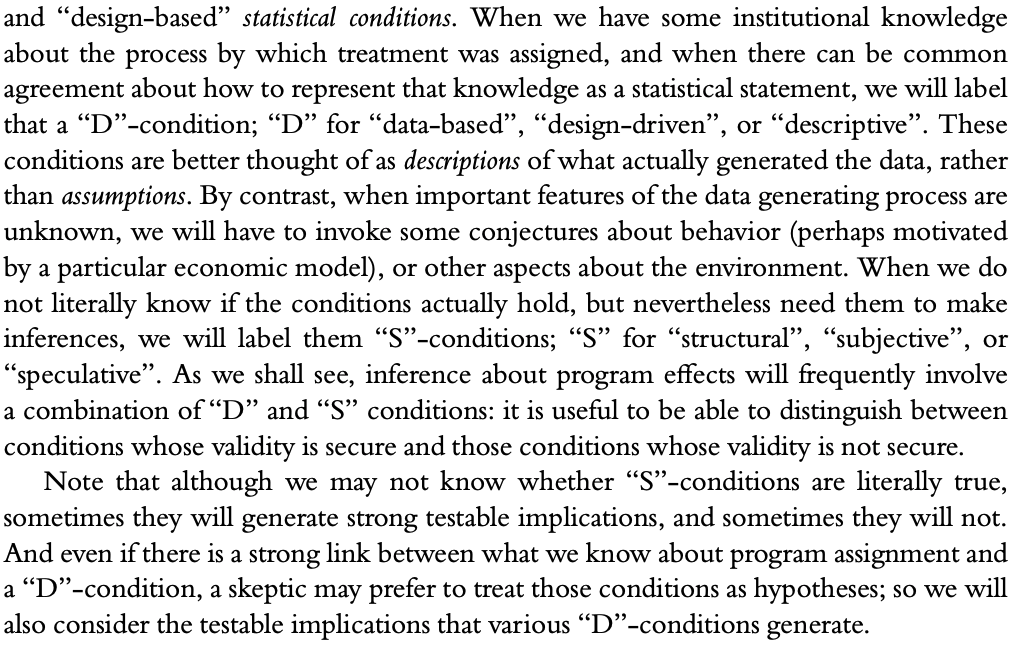
\includegraphics[width=\linewidth]{images/dinardolee.png}}
    \end{column}%
  \end{columns}
\end{frame}


\begin{frame}{Revisiting Research Design}
  \begin{columns}[T] % align columns
    \begin{column}{0.7\textwidth}
      \begin{wideitemize}
      \item D-condition designs fall clearly into the ``PGP''
        description of a research design -- knowledge of the DGP leads
        to a variation in the data generating our identification
      \item S-conditions fall less clearly into this context (as we
        will discuss).
        \begin{itemize}
        \item The relationship between X and Y can be clearly
          articulated, but how it is potentially approximated by a
          random experiment is less obvious
        \end{itemize}
      \item This issue will become clear as we discuss our first topic
      \end{wideitemize}
    \end{column}%
    \hfill%
    \begin{column}{.7\textwidth}

    \end{column}%
  \end{columns}
\end{frame}


\begin{frame}{Estimating causal effects in real settings}
  \begin{columns}[T] % align columns
    \begin{column}{.58\textwidth}
      \begin{wideitemize}
      \item In many applications, we want to estimate the effect of a policy across groups
      \item However, the policy assignment is  \emph{not} necessarily uncorrelated with group characteristics
      \item How can we identify the effect of the policy without being confounded by these level differences?
      \end{wideitemize}
    \end{column}%
    \hfill%
    \begin{column}{.38\textwidth}
      {\onslide<2->
        \vspace{30pt}
      \begin{center}
        \Large \textcolor{red}{Difference-in-differences!}
        \normalsize (DinD)
        \end{center}
        }
    \end{column}%
  \end{columns}
\end{frame}

\begin{frame}{First, a warning}
  \begin{columns}[T] % align columns
    \begin{column}{.99\textwidth}
      \begin{wideitemize}
      \item This literature has had a certain amount of upheaval over the
        past 5-6 years
      \item Tension: provide context for how people currently and
        historically have studied diff-in-diff
        \begin{itemize}
        \item But also elaborate on concerns identified in recent papers
        \end{itemize}
      \item The key issues boil down into two questions:
        \begin{enumerate}
        \item \emph{What is the counterfactual estimand?}
          \begin{itemize}
            \item Does your estimator map to your estimand? (e.g. ``Are you getting at what you meant to?'')
          \end{itemize}
        \item \emph{What are your structural assumptions and their implications?}
          \begin{itemize}
          \item Do you need to assume functional forms? (e.g. ``Is
            this really something that has an experimental analog''?)
          \end{itemize}
        \end{enumerate}
      \item Papers have both pointed out issues but also provided
        solutions to almost all of the problems that they've raised,
        so not something that should prevent you from using these
        tools
      \end{wideitemize}
    \end{column}%
    \hfill%
    \begin{column}{.38\textwidth}
      
    \end{column}%
  \end{columns}
\end{frame}


\begin{frame}{Basic setup }
  \begin{wideitemize}
  \item Assume we have $n$ units ($i$) and $T$ time periods $(t)$
  \item Consider a binary policy $D_{it}$, and we are interested
    in estimating its effect on outcomes $Y_{it}$
  \item The inherent problem is that $D_{it}$ is \emph{not}
    necessarily randomly assigned
  \item The historical key (and parametric) assumption underlying of
    the potential outcomes model (one version):
    \begin{align*}
      Y_{it}(D_{it}) &= \alpha_{i} + \gamma_{t} + \tau_{i}D_{it}\\
      \text{s.t.} &\; Y_{it}(1) - Y_{it}(0)=  \tau_{i}
    \end{align*}
  \item Implication? In the absence of the treatment, the $Y_{it}$
    across units \textbf{evolve in parallel} -- their $\gamma_{t}$ are
    identical. Absent the policy, units may have different
    \emph{levels} ($\alpha_{i}$) but their changes would evolve in
    parallel
    \begin{itemize}
    \item This is a key (parametric!) identifying assumption
    \item $Y_{it}(0) - Y_{i,t-k}(0) = \gamma_{t} - \gamma_{t-k}$, $Y_{it}(0) - Y_{jt}(0) = \alpha_{i} -\alpha_{j}$
    \end{itemize}
  \end{wideitemize}
\end{frame}

\begin{frame}{Basic 2x2 DinD setup}
  \begin{columns}[T] % align columns
    \begin{column}{0.8\textwidth}
      \begin{wideitemize}
      \item Recall our typical estimand of interest is the ATE or the ATT:
        \begin{align*}
          \tau_{ATE} &= E(Y_{it}(1) - Y_{it}(0)) = E(\tau_{i})\\
          \tau_{ATT} &= E(Y_{it}(1) - Y_{it}(0)) = E(\tau_{i} |D_{it} = 1)          
        \end{align*}
      \item Since $D$ is not randomly assigned and we only observe one time
        period, this model is inherently not identified without additional assumptions.
        \begin{itemize}
        \item Why? $D_{i}$ could be correlated with $\alpha_{i}$
        \item Recall that our plug-in estimator approaches need
          estimates for $E(Y_{it}(1))$ and $E(Y_{it}(0))$
        \item Where can we get unbiased estimates?
        \end{itemize}
      \item With two time periods we can make a lot more progress!
        \pause
      \end{wideitemize}
    \end{column}%
    \hfill%
    \begin{column}{.45\textwidth}
    \end{column}%
  \end{columns}
\end{frame}


\begin{frame}{2 $\times$ 2 DinD estimation}
      \begin{center}
        \begin{tabular}{c|cc}
          & t =0 & t = 1\\
          \midrule
          $D = 0$ &  $\gamma_{0} + \alpha_{i}$  & $ \gamma_{1} + \alpha_{i}$\\
          $D = 1$ &  $ \gamma_{0} + \alpha_{i} + \tau_{i} $ & $\gamma_{1} + \alpha_{i} + \tau_{i}$
      \end{tabular}
    \end{center}
    \begin{wideitemize}
    \item Now consider the within unit difference:
      $$Y_{i1} - Y_{i0} = (\gamma_{1} - \gamma_{0}) + \tau_{i}(D_{i1} - D_{i0})$$
    \item Hence 
    \begin{align*}
      E(Y_{i1} - Y_{i0} | D_{i1} - D_{i0} = 1) - E(Y_{i1} - Y_{i0} | D_{i1} - D_{i0} = 0) &= E(\tau_{i}  | D_{i1} - D_{i0} = 1) 
    \end{align*}
  \item Wait, you say, that's a lot more notation than I was expecting.
    \begin{itemize}
    \item Simplifying assumption: treatment only goes one way in
      period 1
    \item  ``absorbing adoption'', e.g. $D_{i0} = 0$
    \end{itemize}
    \begin{align*}
      E(Y_{i1} - Y_{i0} | D_{i1} = 1) - E(Y_{i1} - Y_{i0} | D_{i1} = 0) =  \underbrace{E(\tau_{i}  | D_{i1} = 1) }_{ATT}
    \end{align*}
  \end{wideitemize}
\end{frame}

\begin{frame}{An aside on our simplifying assumption}
  \begin{wideitemize}
  \item The choice of focusing on take-up of a policy, such that $D_{i1} \geq D_{i0}$, is well-grounded in many policy settings
  \item However, there are cases where policies turn on, and then turn off, and this can vary across units
  \item This can be challenging and potentially problematic with
    heterogeneous effects
  \item Need to think carefully about whether $D_{i}$ turning on is
    identical (but opposite sign) to $D_{i}$ turning off
    \begin{itemize}
    \item Hull (2018) working paper on mover designs discusses this
    \end{itemize}
  \item For today, will ignore this issue
  \end{wideitemize}
\end{frame}

\begin{frame}{Estimation using linear regression}
  \begin{wideitemize}
  \item A simple linear regression will identify
    $E(\tau_{i} | D_{i1} = 1)$ with two time periods:
    \begin{equation}
      Y_{it} = \alpha_{i}+ \gamma_{t} + D_{it}\beta + \epsilon_{it}
    \end{equation}
  \item This setup is sometimes referred to as the Two-way Fixed Effects estimator (TWFE)
  \item Note: we could have also estimated $\tau$ directly:
    \begin{align*}
      \hat{\tau} = n^{-1}\sum_{i} \underbrace{D_{i}(Y_{i1} - Y_{i0})}_{\Delta \overline{Y}_{1}} - \underbrace{(1-D_{i1})(Y_{i1} - Y_{i0})}_{\Delta \overline{Y}_{0}}
    \end{align*}
    \begin{itemize}
    \item Intuitively, we generate a counterfactual for the treatment
      using the changes in the untreated units: $E(Y_{i1} - Y_{i0} | D_{i}=0)$
    \end{itemize}
  \item Necessary: two time periods! What if we have more?
  \end{wideitemize}
\end{frame}

\begin{frame}{Multiple time periods in basic setup}
  \begin{wideitemize}
  \item Let's consider a policy that occurs all at $t_{0}$
    (e.g. single timing rolled out to treated units)
  \item  More time periods helps in several ways:
    \begin{enumerate}
    \item If we have multiple periods \emph{before} the policy implementation, we can partially test the underlying assumptions
      \begin{itemize}
      \item Sometimes referred to as ``pre-trends''
      \end{itemize}
    \item If we have multiple periods \emph{after} the policy implementation, we can examine the timing of the effect
      \begin{itemize}
      \item Is it an immediate effect? Does it die off? Is it persistent?
      \item If you pool all time periods together into one ``post'' variable, this estimates the average effect. If sample is not balanced, can have unintended effects!
      \end{itemize}
    \end{enumerate}
  \item  How do we implement this? 
    \begin{equation*}
      Y_{it} = \alpha_{i} + \gamma_{t} + \sum_{t=1, t\not=t_{0}}^{T}\delta_{t} D_{it} + \epsilon_{it},
    \end{equation*}
    \begin{itemize}
    \item One of the coefficients is fundamentally unidentified
      because of $\alpha_{i}$
    \item All coefficients measure the effect \emph{relative} to period $t_{0}$.
      \end{itemize}
  \end{wideitemize}
\end{frame}

\begin{frame}{Pre-testing and structural assumptions}
  \begin{wideitemize}
  \item Note that for the above model, we made a stronger assumption about trends
    \begin{itemize}
    \item  The Dinardo and Lee ``S-assumptions'' start to bite
    \item We assumed that
      $Y_{it}(d) - Y_{i,t-k}(d) = \gamma_{t} - \gamma_{t-k}$ for all
      $k$ and $d$
    \item This is testable pre-treatment (hence the pre-test)
    \end{itemize}
  \item This is very powerful and has helped spark the growth in DinD regressions
    \begin{itemize}
    \item Visual demonstrate of ``pre-trends'' helps support the
      validity of the design
    \item Worth doing!
    \end{itemize}
  \item Two key issues:
    \begin{enumerate}
    \item Pre-testing can cause statistical problems
    \item What does parallel trends even mean?
    \end{enumerate}
  \end{wideitemize}
\end{frame}

\begin{frame}{Pre-testing issues (Roth 2020)}
  \begin{columns}[T] % align columns
    \begin{column}{0.5\textwidth}
      \begin{wideitemize}
      \item Consider $T = 3$ and think about what a pre-trend test is
        trying to do
      \item Testing whether the difference relative to $t= 0$ for $t=-1$ is significant
      \item<3-> Unconditionally, this is reasonable. However, Roth
        (2020) highlights that this is a form of \emph{pre-testing},
        and that low power in detecting pre-trends can be problematic
      \item<5-> By selecting on pre-trends that ``pass'', will tend to
        choose baseline realizations that satisfy pre-trends, but
        induce \emph{bias} in the effect
      \end{wideitemize}
    \end{column}%
    \hfill%
    \begin{column}{.5\textwidth}
      \only<1>{      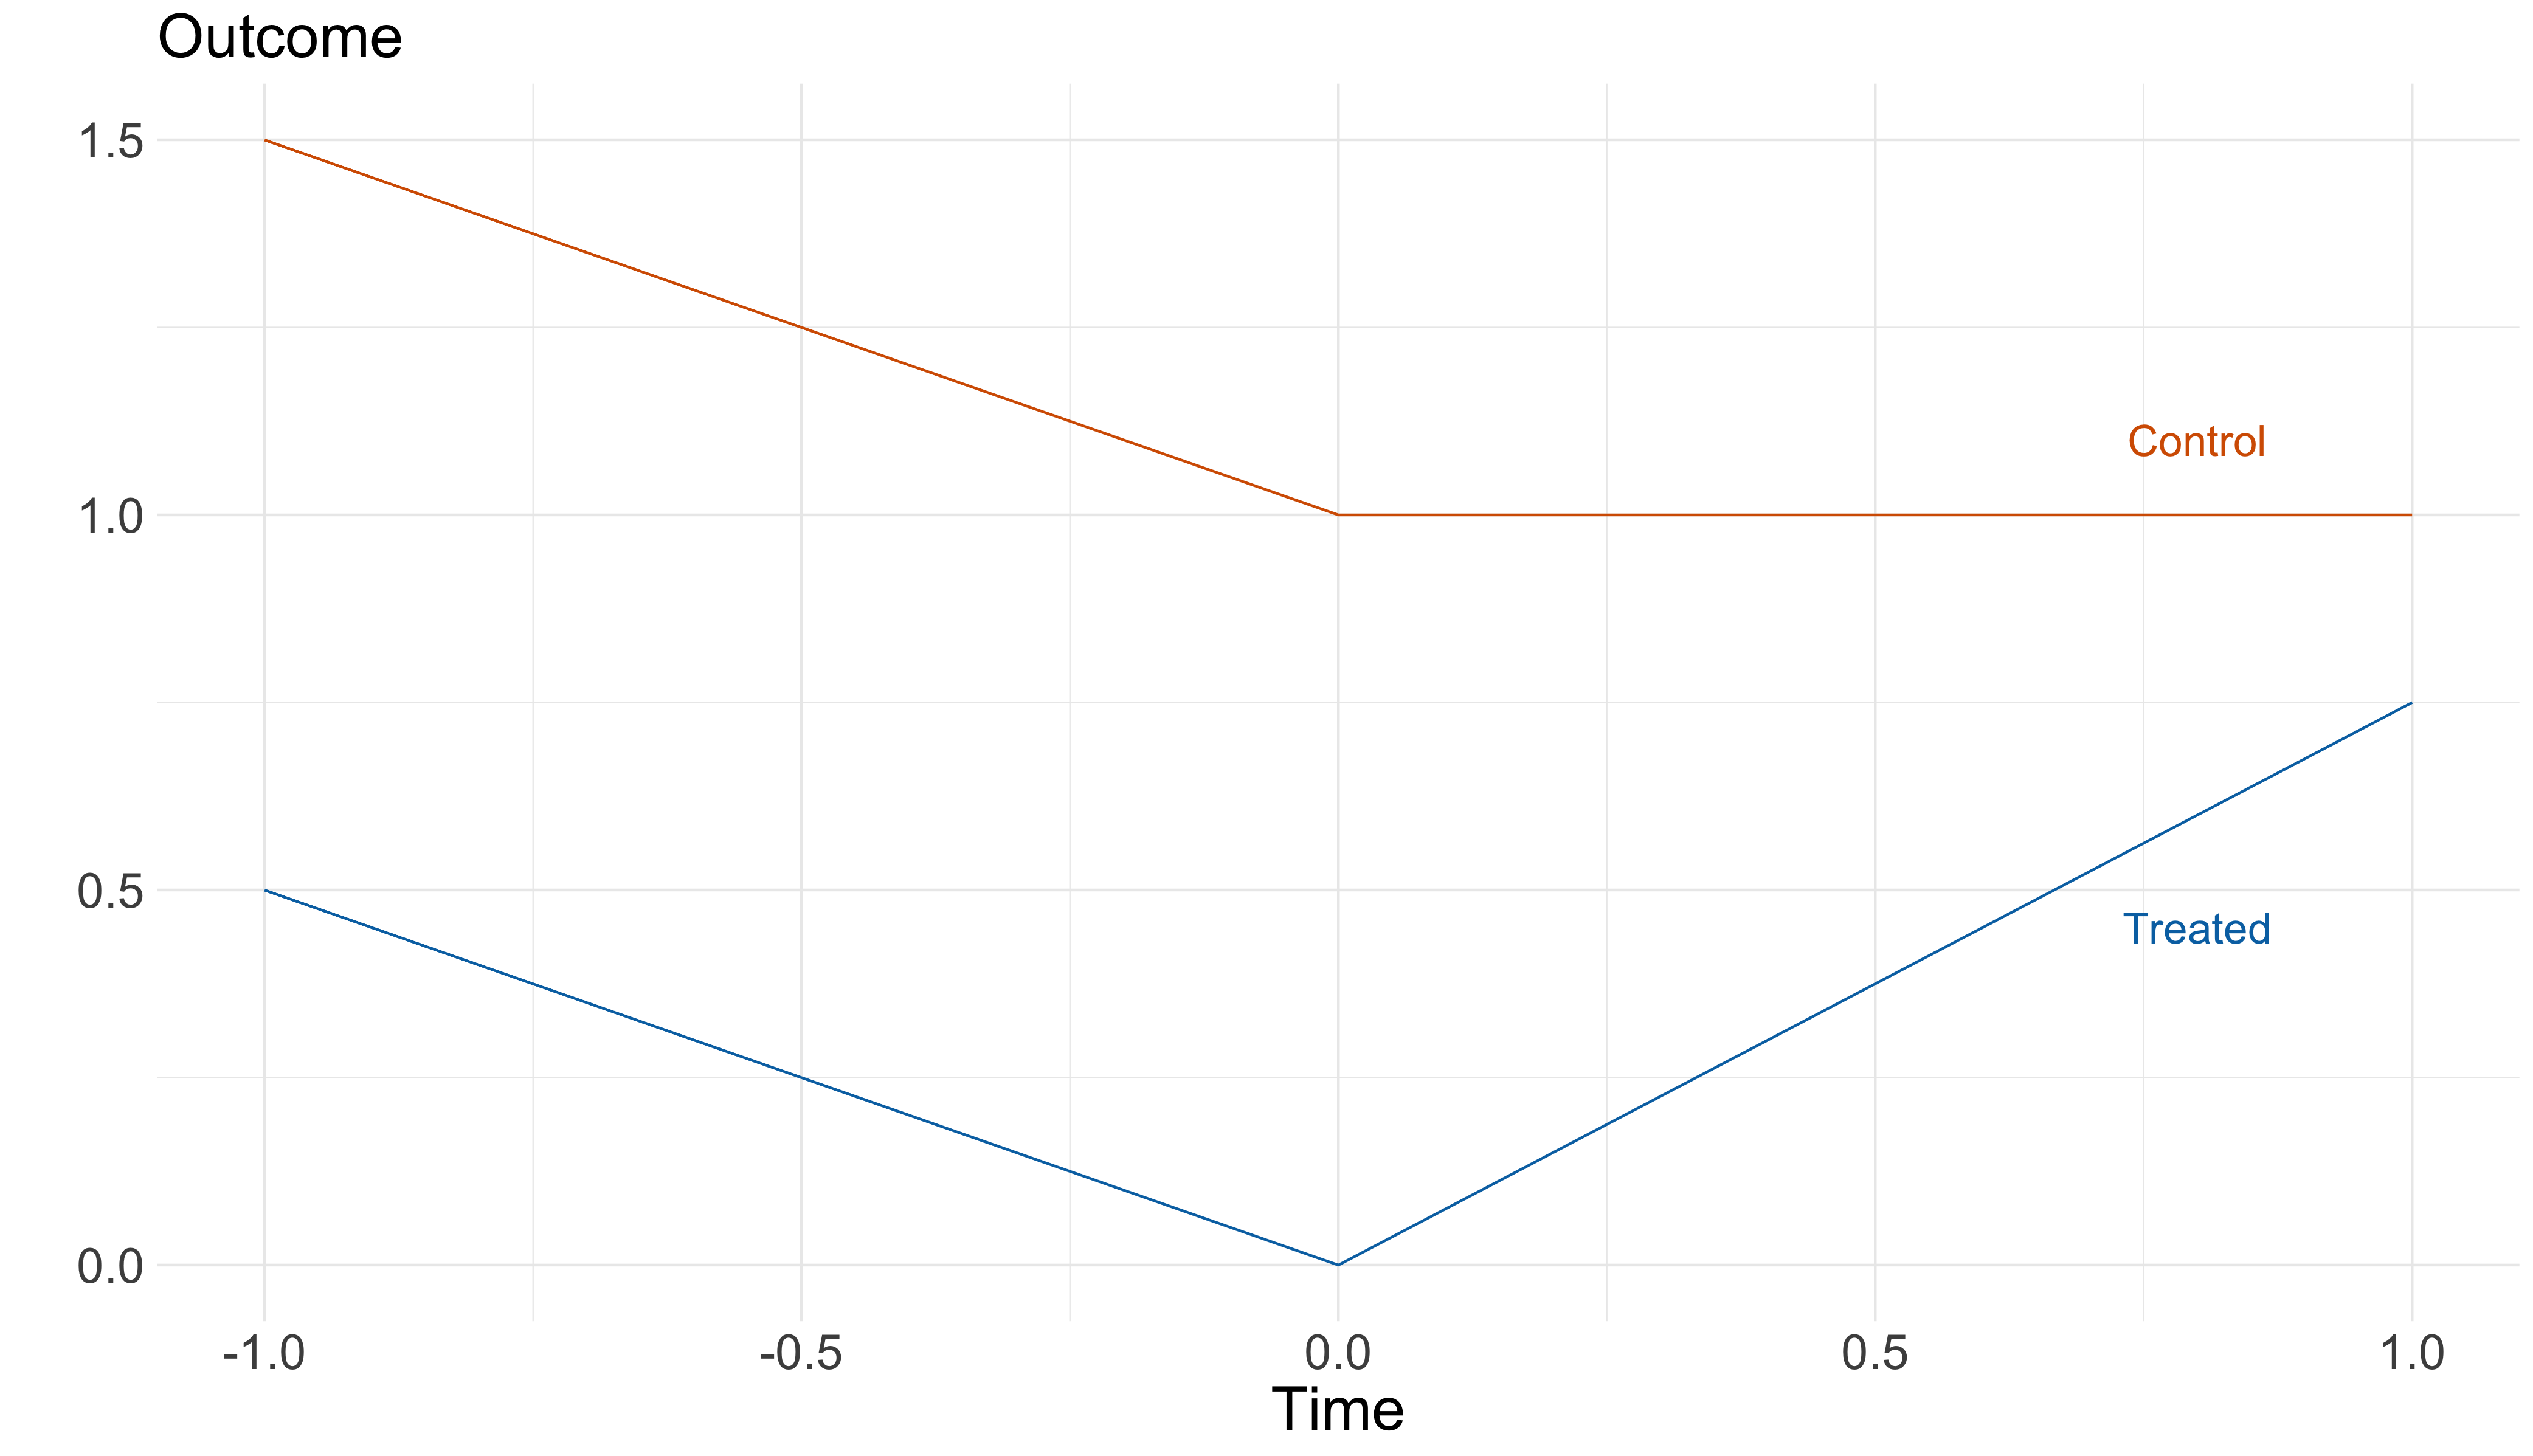
\includegraphics[width=\linewidth]{images/rothpic1.png}}
      \only<2>{      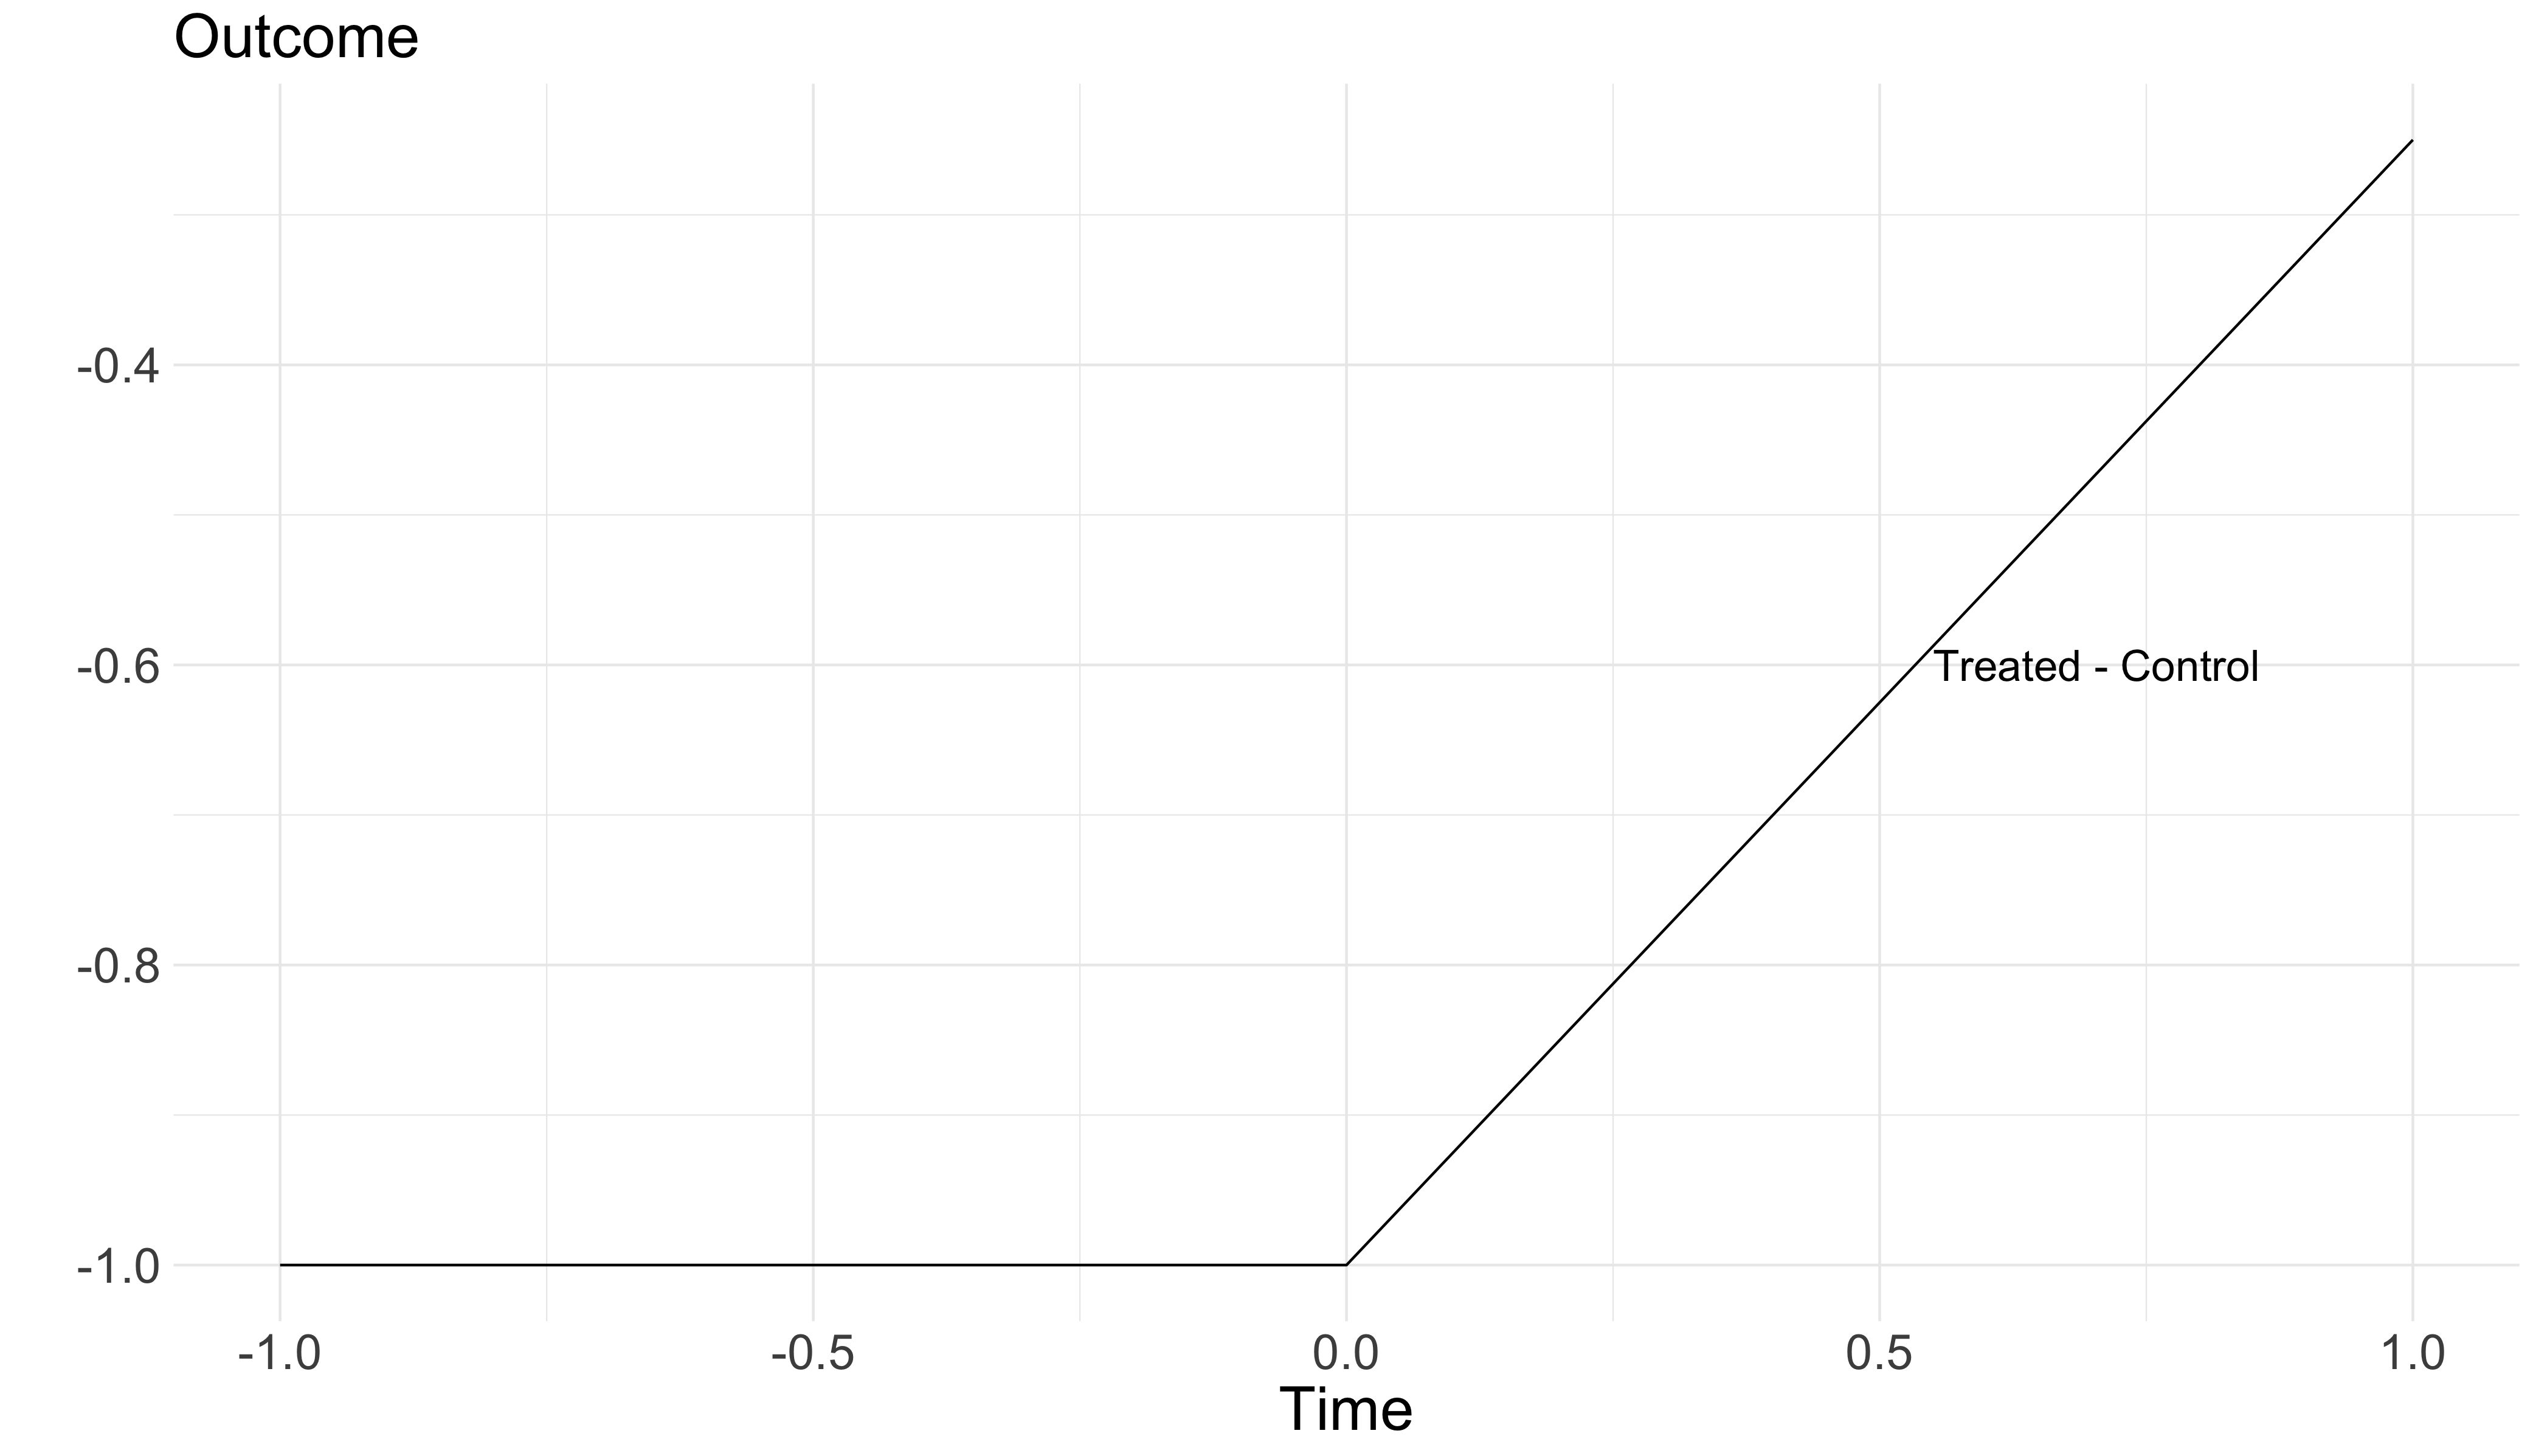
\includegraphics[width=\linewidth]{images/rothpic2.png}}
      \only<3>{      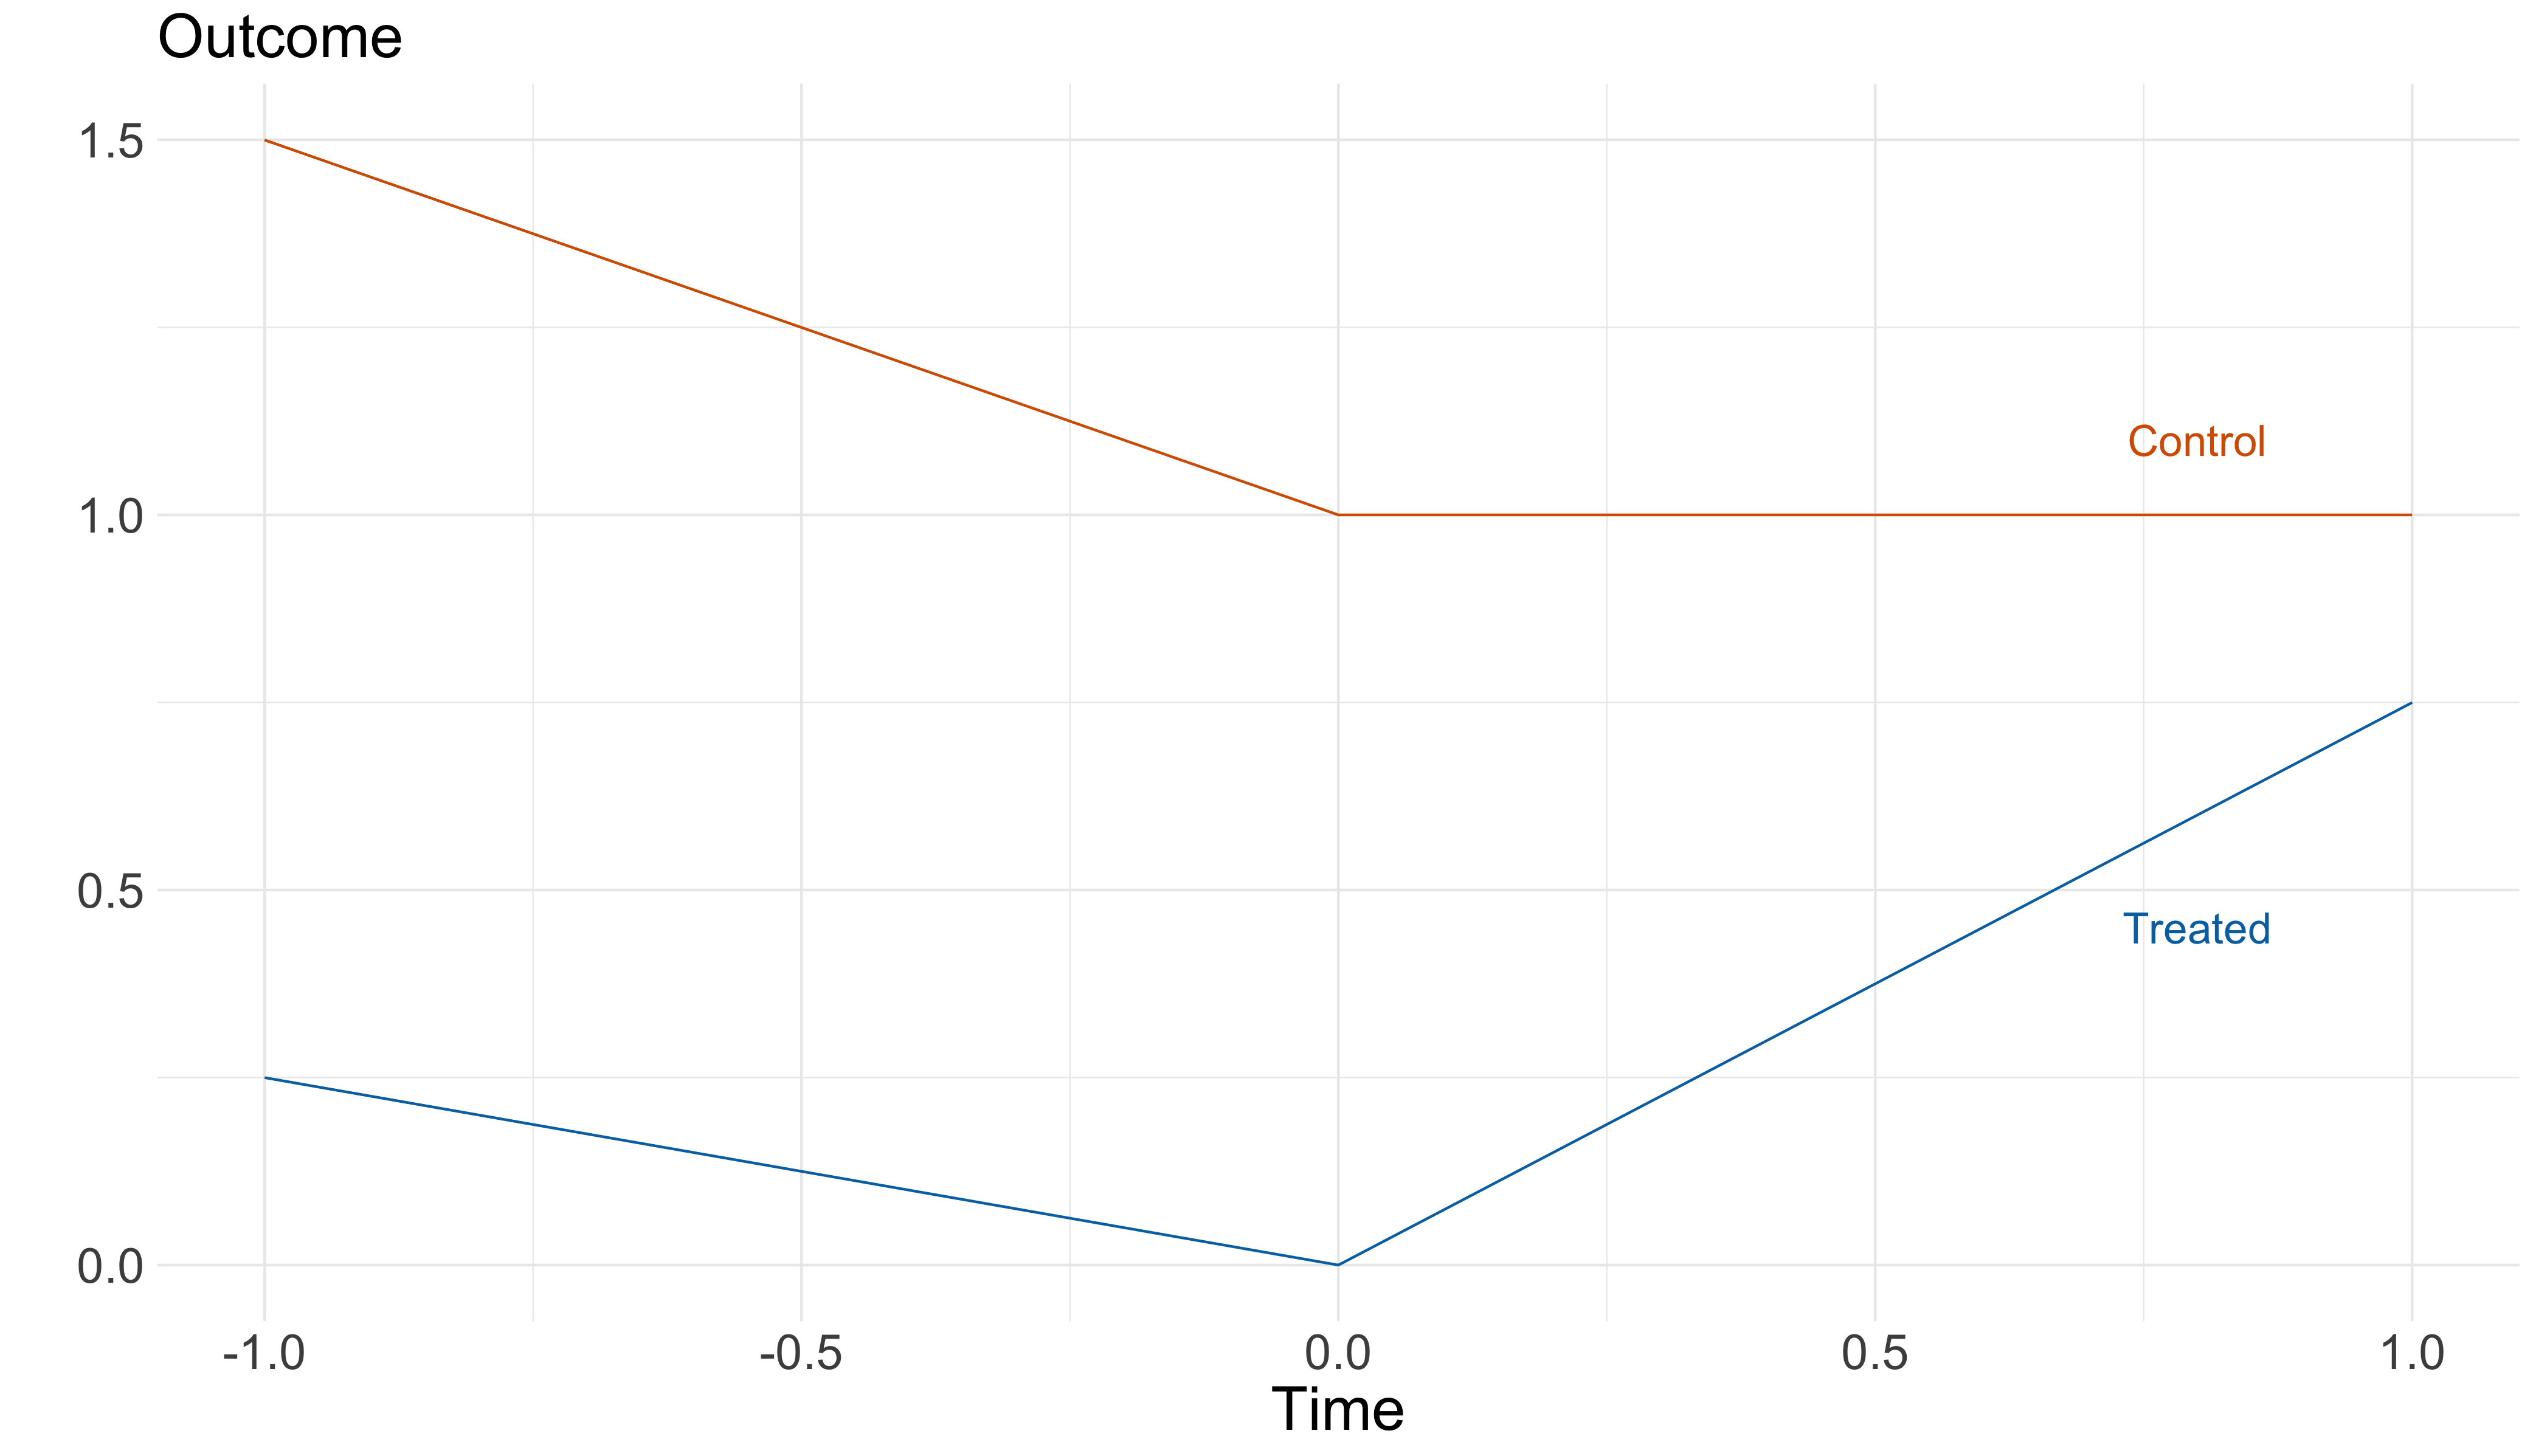
\includegraphics[width=\linewidth]{images/rothpic3.png}}
      \only<4>{      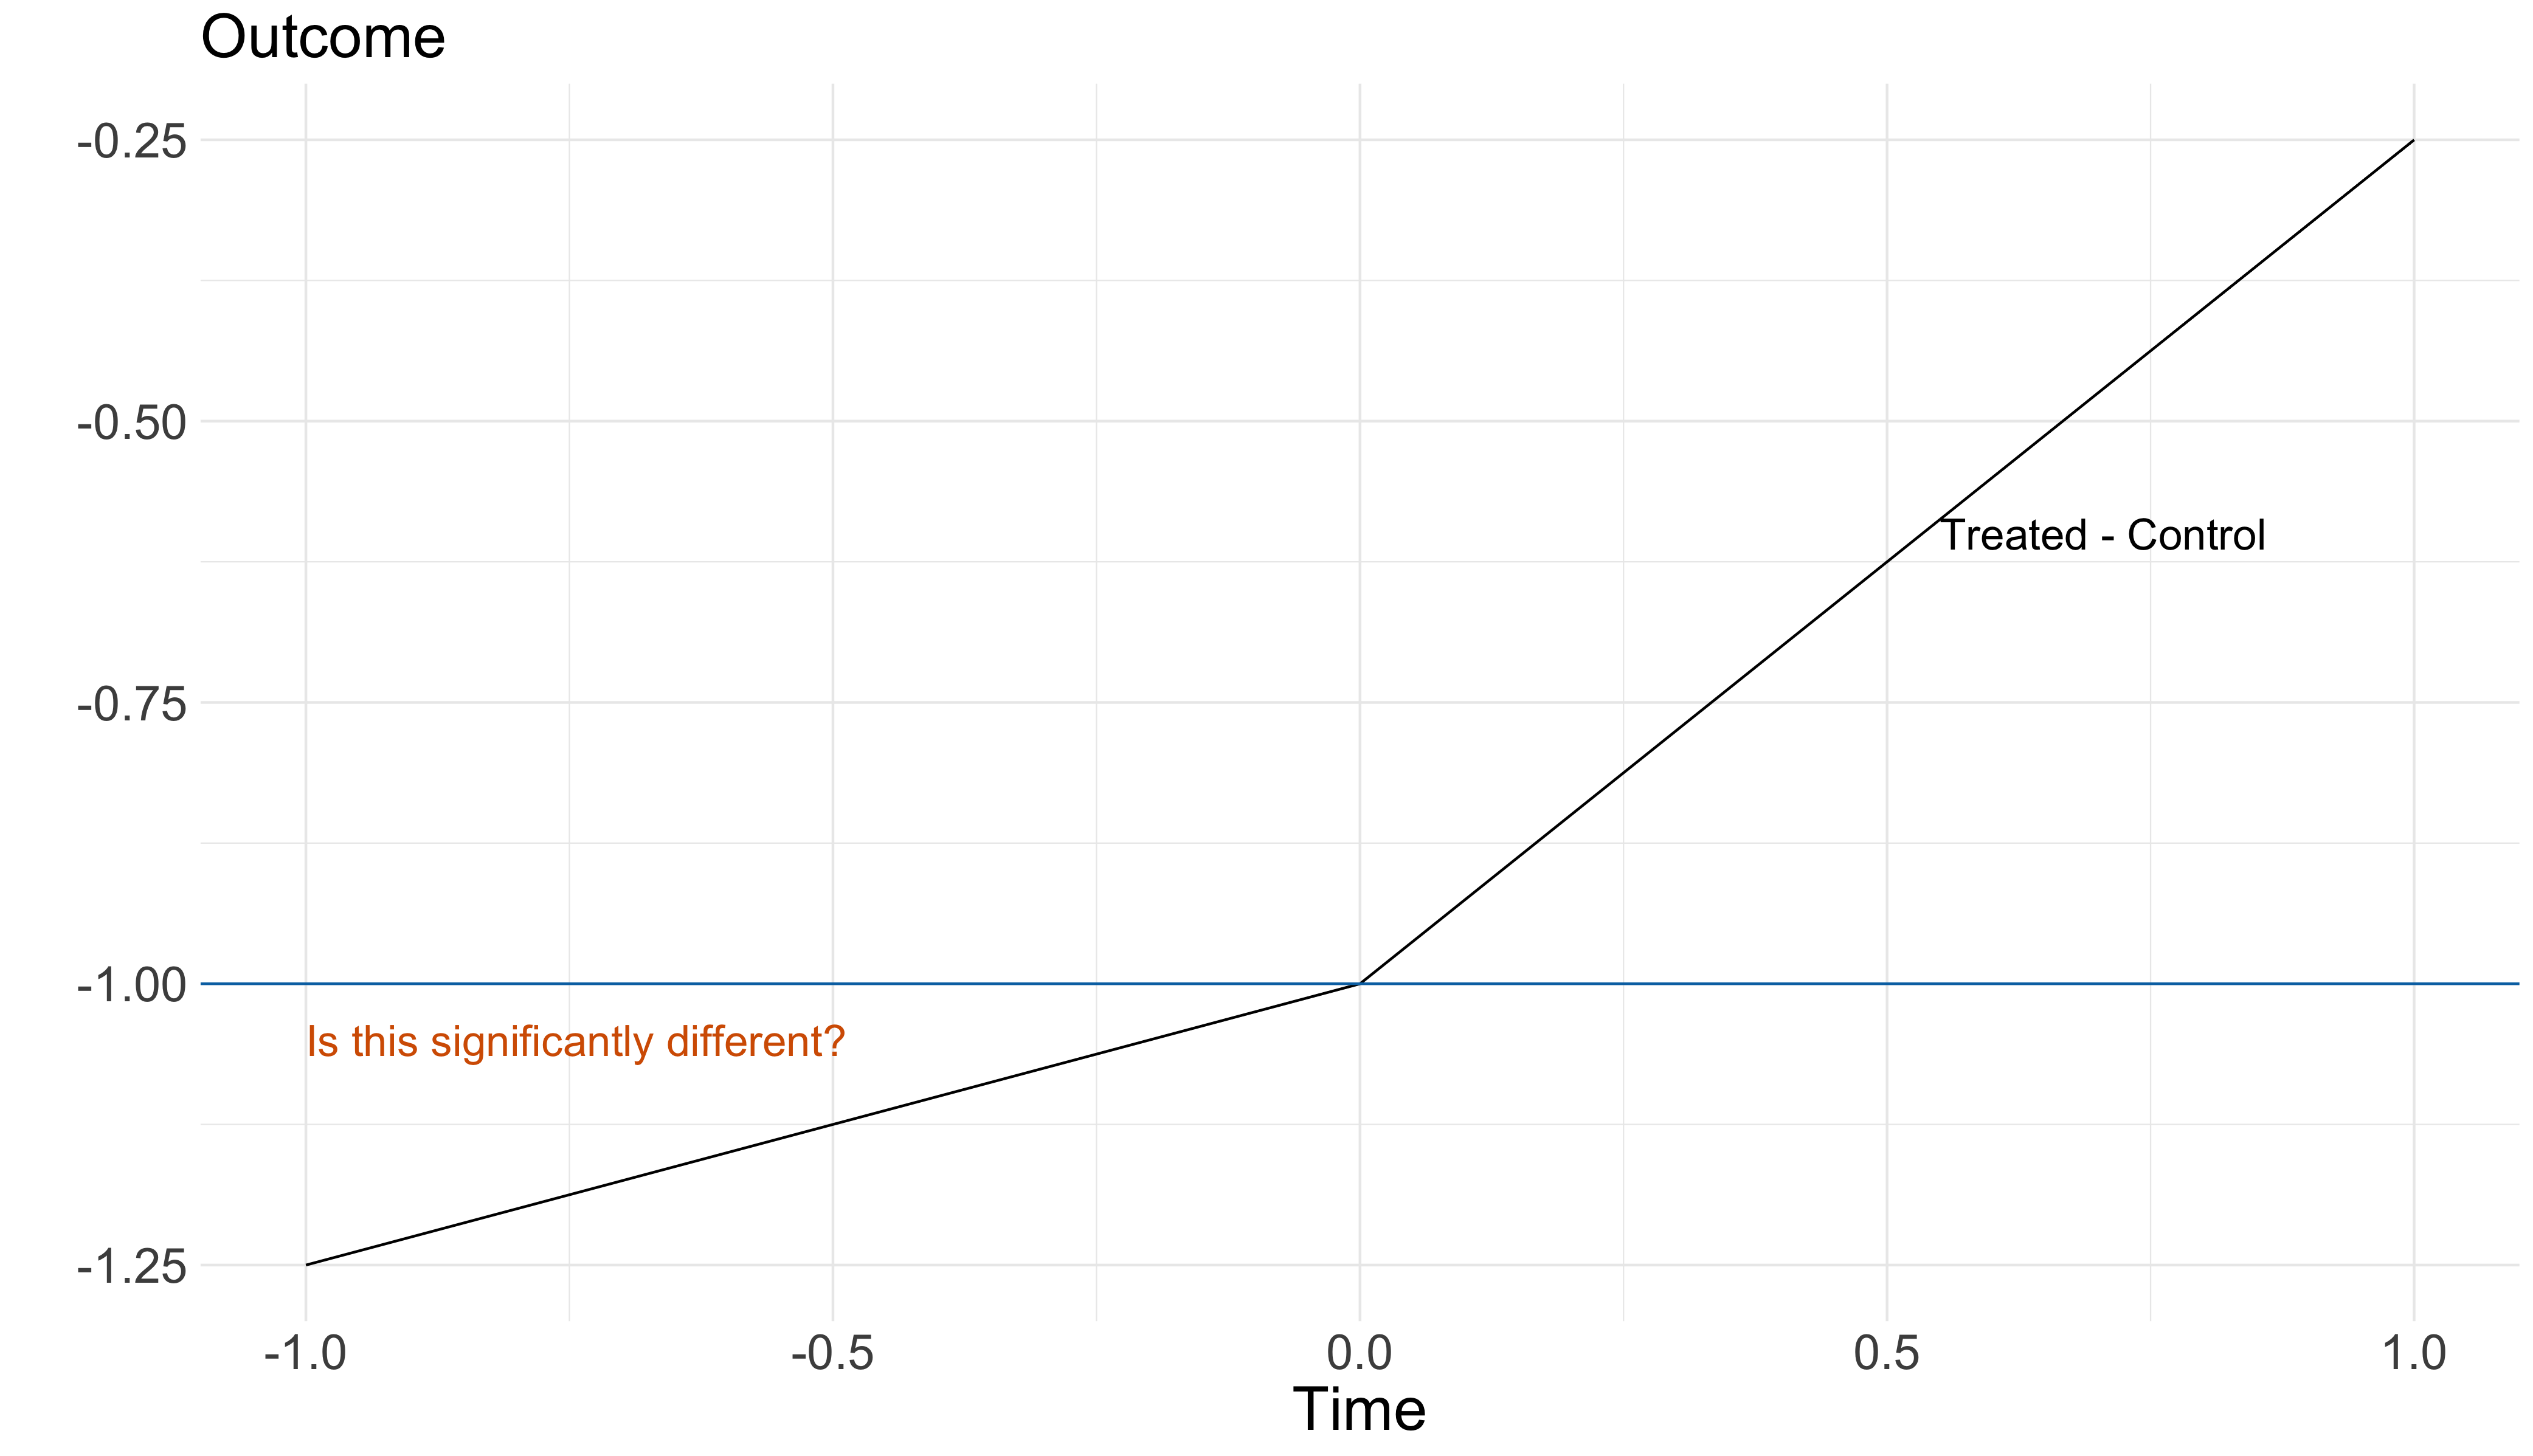
\includegraphics[width=\linewidth]{images/rothpic4.png}}
      \only<5>{      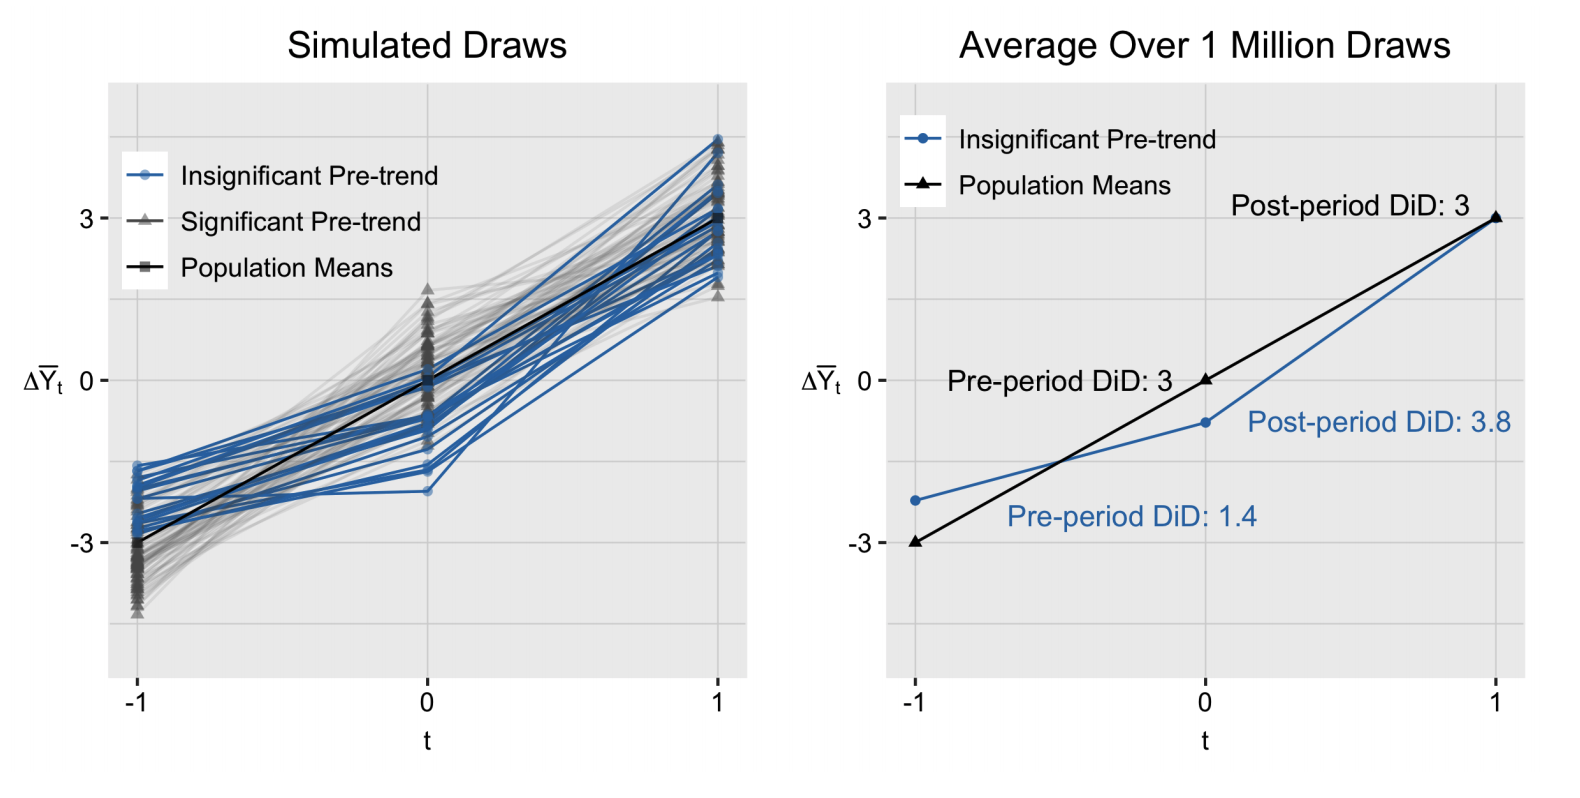
\includegraphics[width=\linewidth]{images/rothpic5.png}}                        
    \end{column}
  \end{columns}
\end{frame}

\begin{frame}{How to interpret this caution?}
  \begin{wideitemize}
  \item First, don't panic. Examining pre-trend is still important
    diagnostic
  \item Important to realize that selecting your design based on
    pre-trend is \emph{constructing} your counterfactual
    \begin{itemize}
    \item Pre-tests will cause you to potentially contaminate your
      design
    \end{itemize}
  \item Suggested solution from Roth (2020): incorporate robustness to
    pre-trends into your analysis. Rambachan and Roth (2020) present
    results on testing sensitivity of DinD results to pre-trends
    \begin{itemize}
    \item Brief intuition follows
    \end{itemize}
  \end{wideitemize}
\end{frame}


\begin{frame}{Rambachan and Roth (2020) suggestion}
  \begin{wideitemize}
  \item Intuitive proposed solution for robustness. Note the post and pre effects:
    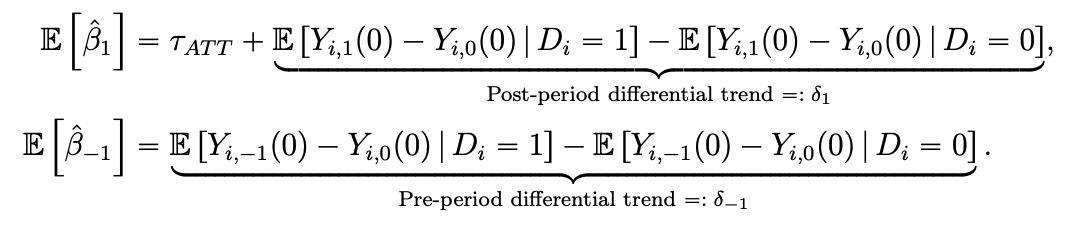
\includegraphics[width=0.7\linewidth]{images/rothpic6.png}
    \vspace{-10pt}
  \item parallel trends assumes these $\delta$ are zero. But pre-trends may not be zero. 
    \begin{itemize}
    \item R\&R say: we can use the info from our pre-trends to bound
      post-trend
    \item Use a \emph{smoothness} assumption, $M$, on the second derivative. E.g. simple case:
    \end{itemize}
    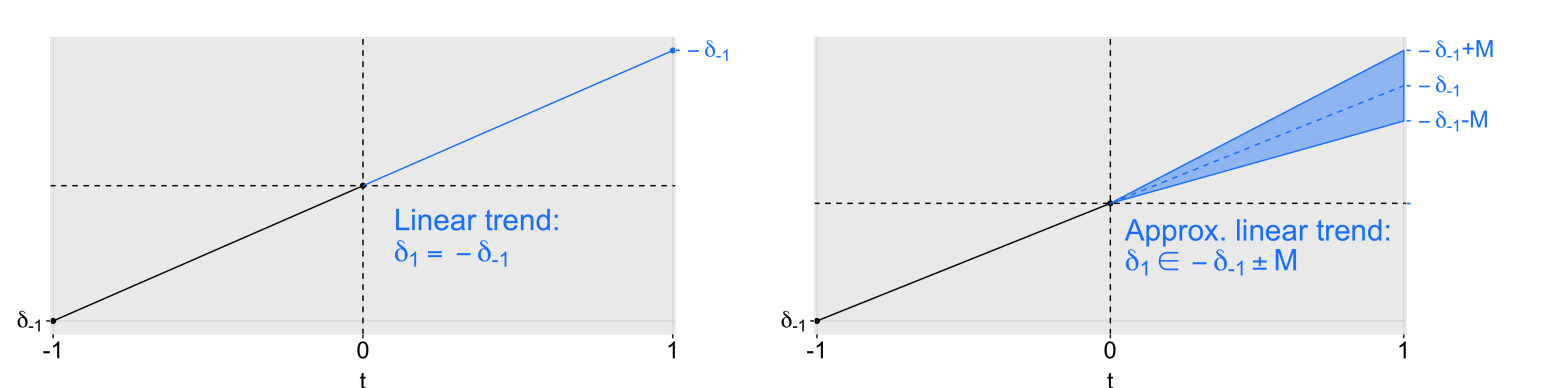
\includegraphics[width=\linewidth]{images/rothpic7.png}    
  \end{wideitemize}
\end{frame}

\begin{frame}{This approach adds more work but also more validity}
  \begin{wideitemize}
  \item  Need to select $M$, and will likely have less strong results
  \item However, very powerful way to address concerns about pre-trends
  \item Code for applying this technique is availabe in R:
    \url{https://github.com/asheshrambachan/HonestDiD}
  \end{wideitemize}
\end{frame}

\begin{frame}{Parallel trends in what?}
  \begin{wideitemize}
  \item A known issue that was historically not formalized is the
    question of what the outcome is specified as: logs, or levels?
  \item Hopefully it's clear that if something satisfies pre-trends in
    logs, it seems unlikely to satisfy in levels
  \item Recall that this is the issue of \emph{invariance} we
    discussed with quantile treatment effects
    \begin{itemize}
    \item In our parametric setting, if there are time trends in the
      outcomes, the parallel trends are likely not to hold for all
      transformations of the variables.
    \item That could be problematic if you wanted to be agnostic about
      the model!
    \end{itemize}
  \item Roth and Sant'Anna (2021) directly discuss this issue. Their suggestion:
    \begin{quote}
      Our results suggest that researchers who wish to point-identify
      the ATT should justify one of the following: (i) why treatment
      is as-if randomly assigned, (ii) why the chosen functional form
      is correct at the exclusion of others, or (iii) a method for
      inferring the entire counterfactual distribution of untreated
      potential outcomes.
    \end{quote}
  \end{wideitemize}
\end{frame}


\begin{frame}{Cases of DinD}
  \begin{columns}[T] % align columns
    \begin{column}{.58\textwidth}
      \begin{wideitemize}
      \item 1 treatment timing, Binary treatment, 2 periods
        \begin{itemize}
        \item Card and Krueger  (AER, 1994)
        \end{itemize}
      \item 1 treatment timing, Binary treatment, T periods
        \begin{itemize}
        \item Yagan (AER, 2015) 
        \end{itemize}
      \item 1 treatment timing, Continuous treatment
        \begin{itemize}
        \item Berger, Turner and Zwick (JF, 2020)
        \end{itemize}
      \item Staggered treatment timing, Binary treatment
        \begin{itemize}
          \item Bailey and Goodman-Bacon (AER, 2015)
        \end{itemize}
      \end{wideitemize}
    \end{column}%
    \hfill%
    \begin{column}{.38\textwidth}
      % \makebox[\linewidth][c]{
      % \resizebox{\linewidth}{!}{
      % \includegraphics{how-to-draw-an-owl.pdf}
      % }
      % }
    \end{column}%
  \end{columns}
\end{frame}


\begin{frame}{Card and Krueger (1994)}
  \begin{wideitemize}
  \item Card and Krueger (1994) study the impact of New Jersey
    increasing the minimum wage 4.25 to 5.05 dollars an hour on April
    1, 1992
  \item Key question is what impact does this have on employment?
    \begin{itemize}
    \item Need a counterfactual for NJ, and use Pennsyvania as a control
    \end{itemize}
  \item Collected data in 410 fast food restaurants
    \begin{itemize}
    \item Called places and asked for employment and starting wage data
    \item Sample data from Feb 1992 and Nov 1992
    \end{itemize}
  \item Hence, $D_{i}$ is NJ vs PA, and $t=0$ is Feb 1992 and $t = 1$ is Nov 1992
  \end{wideitemize}
\end{frame}

\begin{frame}{Stark Effect on Wages in Card and Krueger (1994) }
  \begin{center}
    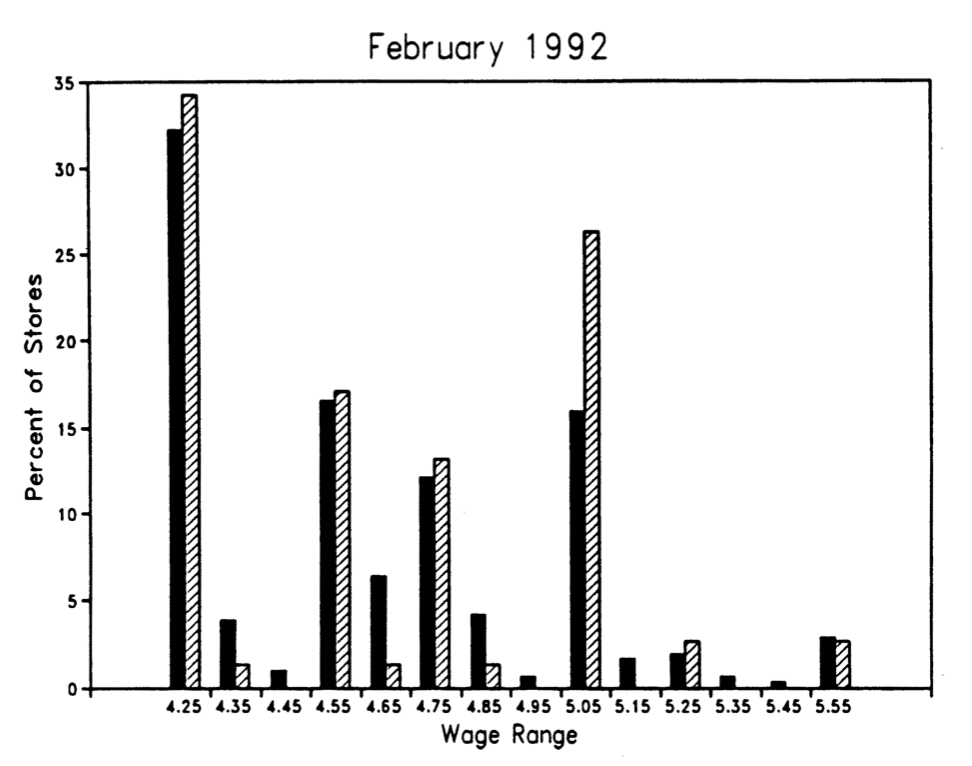
\includegraphics[width=0.45\linewidth]{images/cardkrueger1.png}   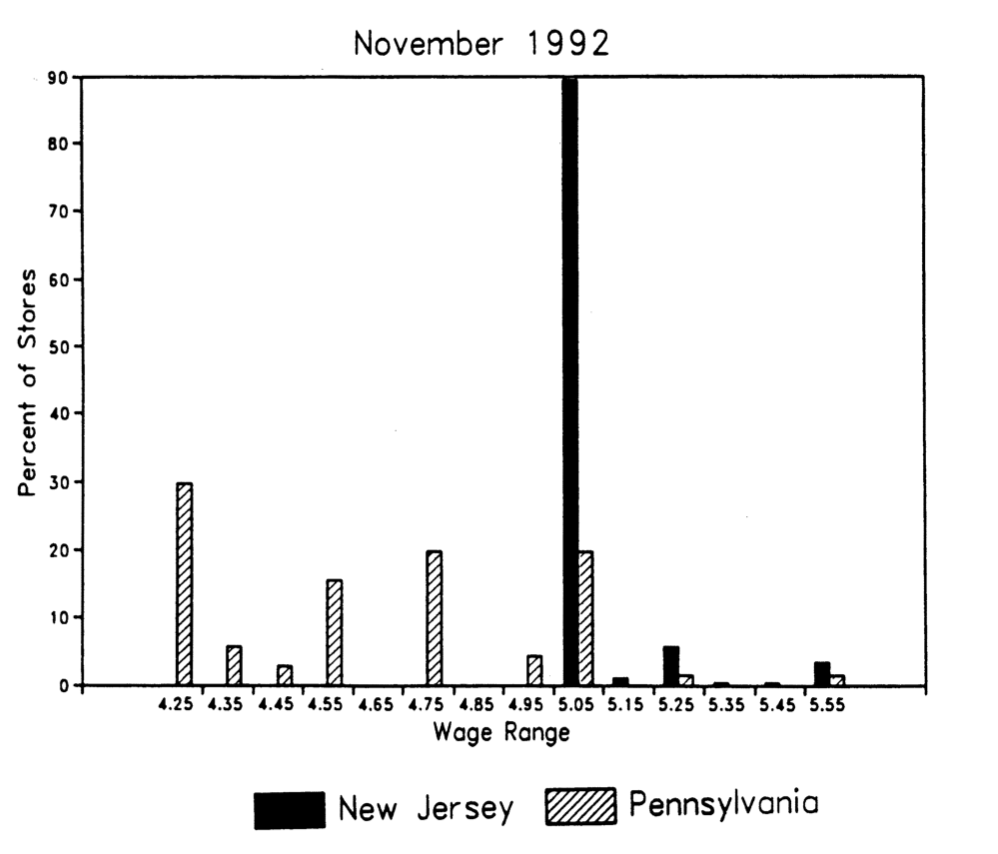
\includegraphics[width=0.45\linewidth]{images/cardkrueger2.png}
    \end{center}
\end{frame}


\begin{frame}{Effect on Employment in Card and Krueger (1994) }
  \begin{columns}[T] % align columns
    \begin{column}{0.5\textwidth}
      \begin{wideitemize}
      \item Despite a large increase in wages, seemingly no negative
        impact on employment
        \begin{itemize}
        \item In fact, marginally significant positive impact
        \end{itemize}
      \item Looking at raw data, this positive impact is driven by a
        decline in PA
        \begin{itemize}
        \item This decline is reasonable if you think that PA is a
          good counterfactual, since 1992 is in the middle of a recession
        \end{itemize}
      \item A second comparison can be run with stores whose starting
        wage in pre-period was above treatment cutoff
        \begin{itemize}
        \item These stores perform similarly to PA
        \end{itemize}
      \end{wideitemize}
    \end{column}%
    \hfill%
    \begin{column}{.5\textwidth}
      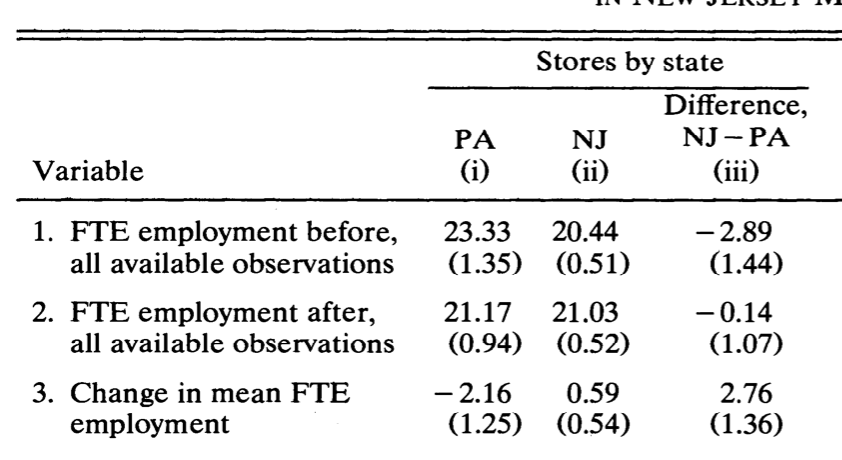
\includegraphics[width=\linewidth]{images/cardkrueger3.png}\\
\hfill      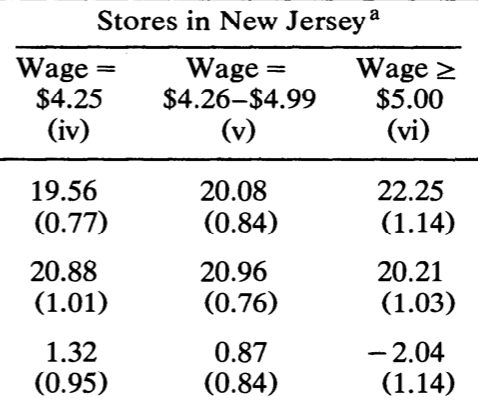
\includegraphics[width=0.5\linewidth]{images/cardkrueger4.png}
    \end{column}%
  \end{columns}
\end{frame}

\begin{frame}{Key considerations for thinking about Card and Krueger (1994)}
  \begin{wideitemize}
  \item The treatment can't really be thought of as randomly assigned
    \begin{itemize}
    \item Treatment is completely correlated within states
    \item As a result, any within-state correlation of errors will be
      correlated with treatment status
    \end{itemize}

  \item Given the limited number of states, time periods, and
    treatments, more valuable to view this as a case study
    \begin{itemize}
    \item Under strong parametric assumptions, can infer causality!
      \item Card acknowledges (Card and Krueger interview with Ben Zipperer):
    \end{itemize}
    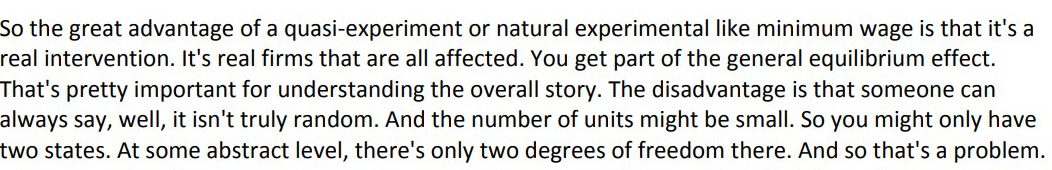
\includegraphics[width=\linewidth]{images/card_interview.png}
  \end{wideitemize}
\end{frame}

\begin{frame}{Yagan (2015)}
  \begin{wideitemize}
  \item Yagan (2015) tests whether the 2003 dividend tax cut
    stimulated corporate investment and increased labor earnings
  \item Big empirical question for corporate  finance and public finance
  \item No direct evidence on the real effects of dividend tax cut
    \begin{itemize}
    \item real corporate outcomes are too cyclical to distinguish tax
      effects from business cycle effects, and economy boomed
    \end{itemize}
  \item Paper uses distinction between ``C'' corp and ``S'' corp designation to estimate effect
    \begin{itemize}
    \item Key feature of law: S-corps didn't have dividend taxation
    \end{itemize}
  \item Identifying assumption (from paper):
    \begin{quote}
      The identifying assumption underlying this research design is
      not random assignment of C- versus S-status; it is that C- and
      S-corporation outcomes would have trended similarly in the
      absence of the tax cut.
    \end{quote}
  \end{wideitemize}
\end{frame}

\begin{frame}{Investment Effects (none)}
      \makebox[\linewidth][c]{
      \resizebox{\linewidth}{!}{
      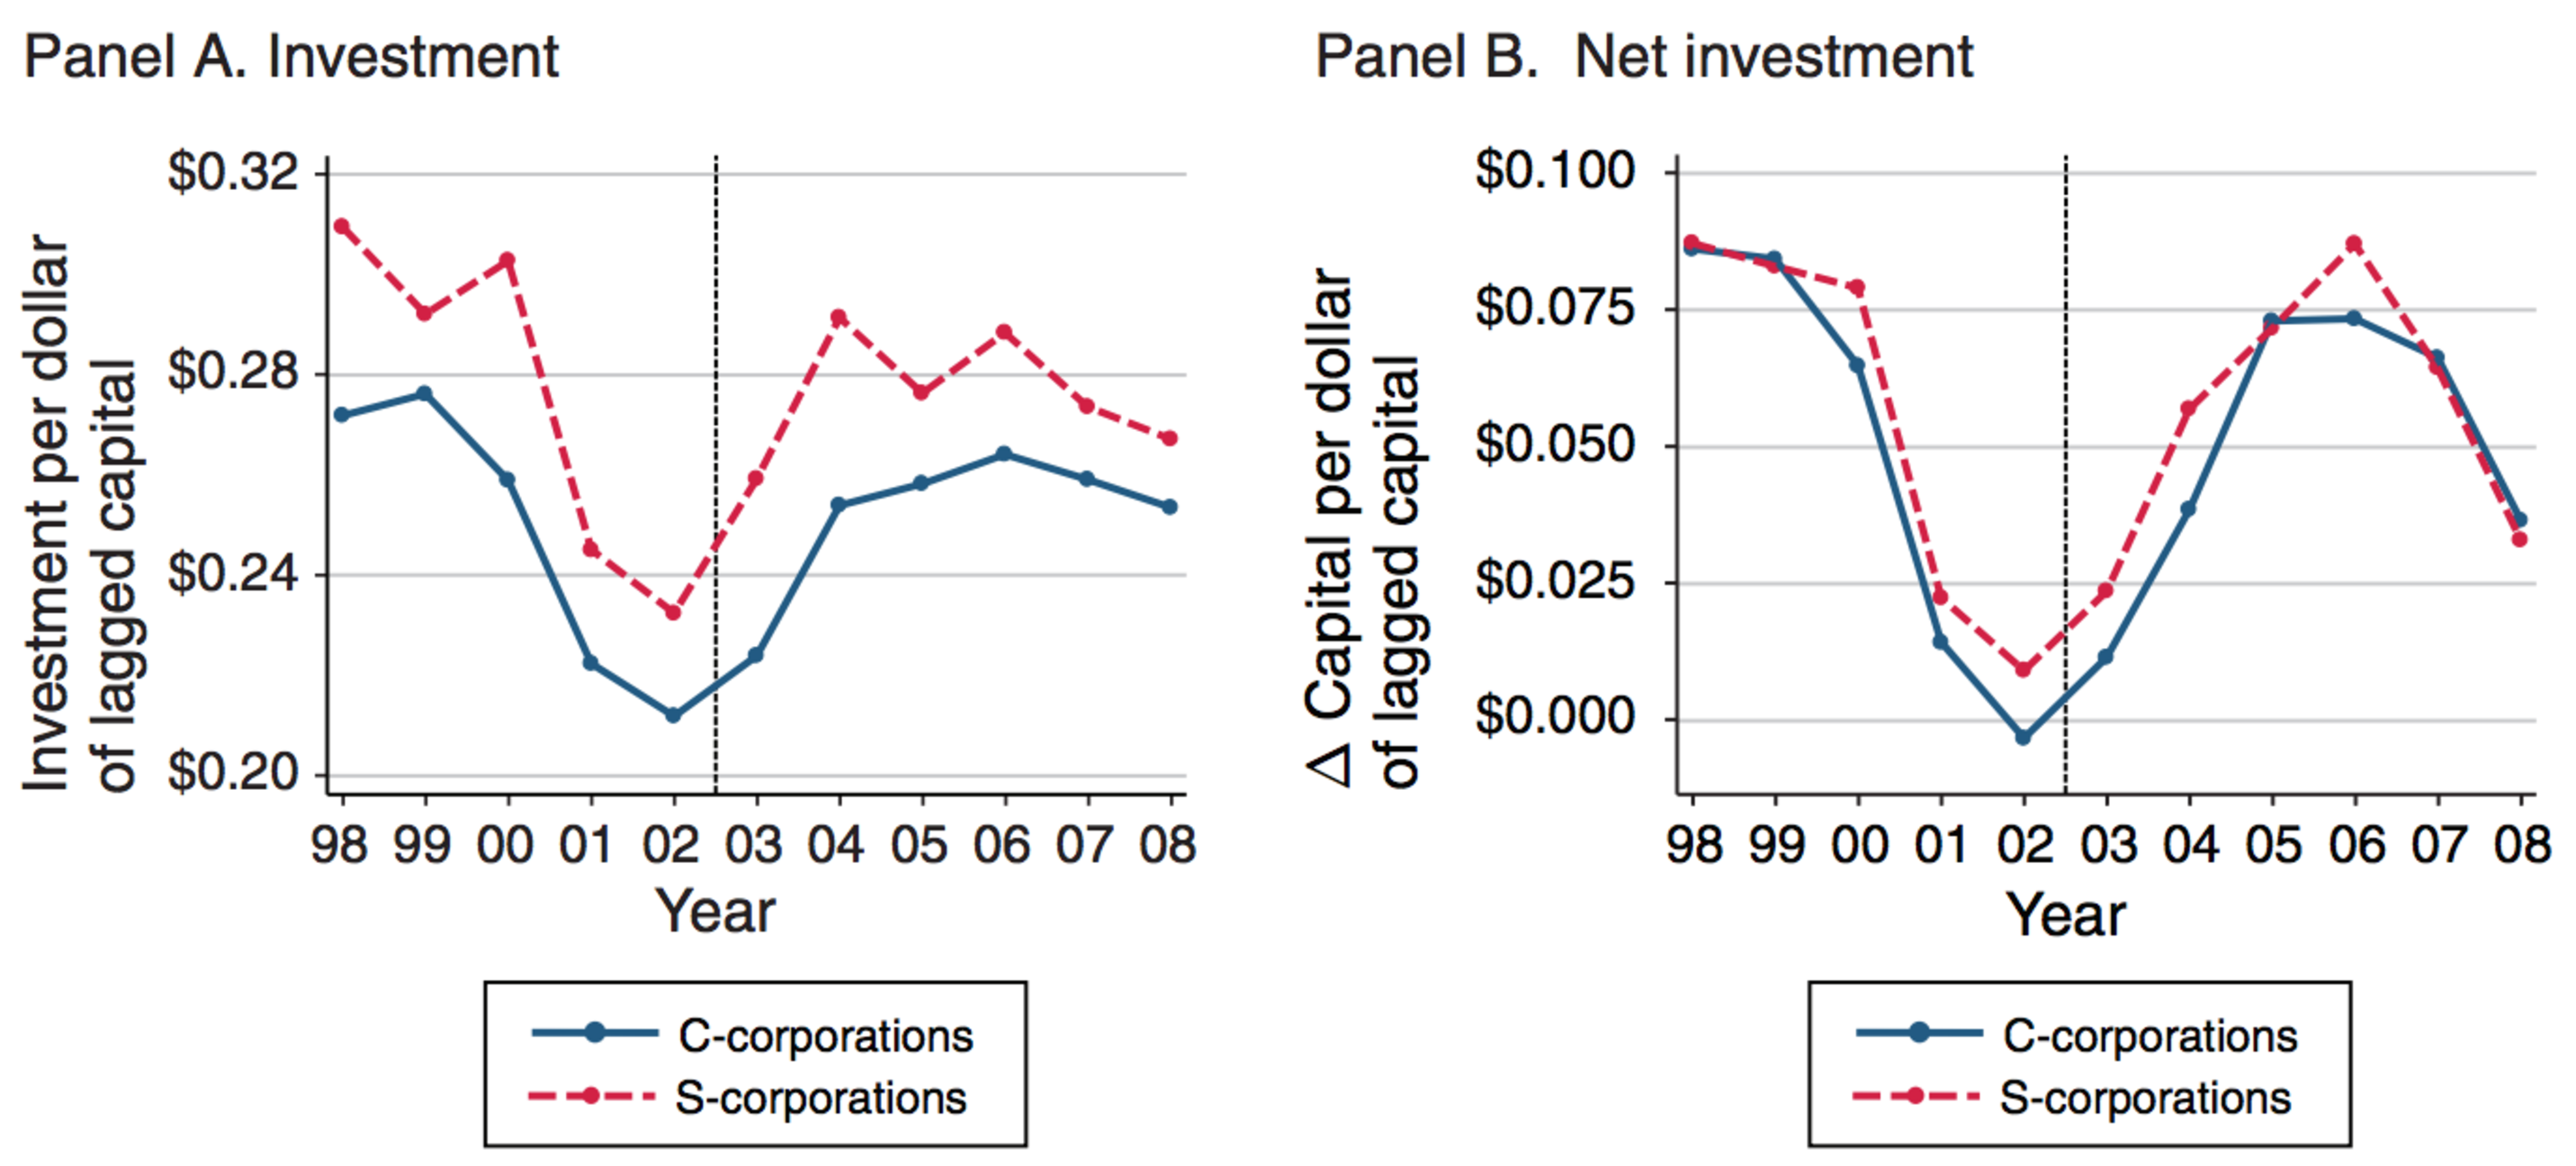
\includegraphics{images/yagan_1.pdf}
      }
      }
\end{frame}
\begin{frame}{Employee + Shareholder effects (big)}
      \makebox[\linewidth][c]{
      \resizebox{\linewidth}{!}{
      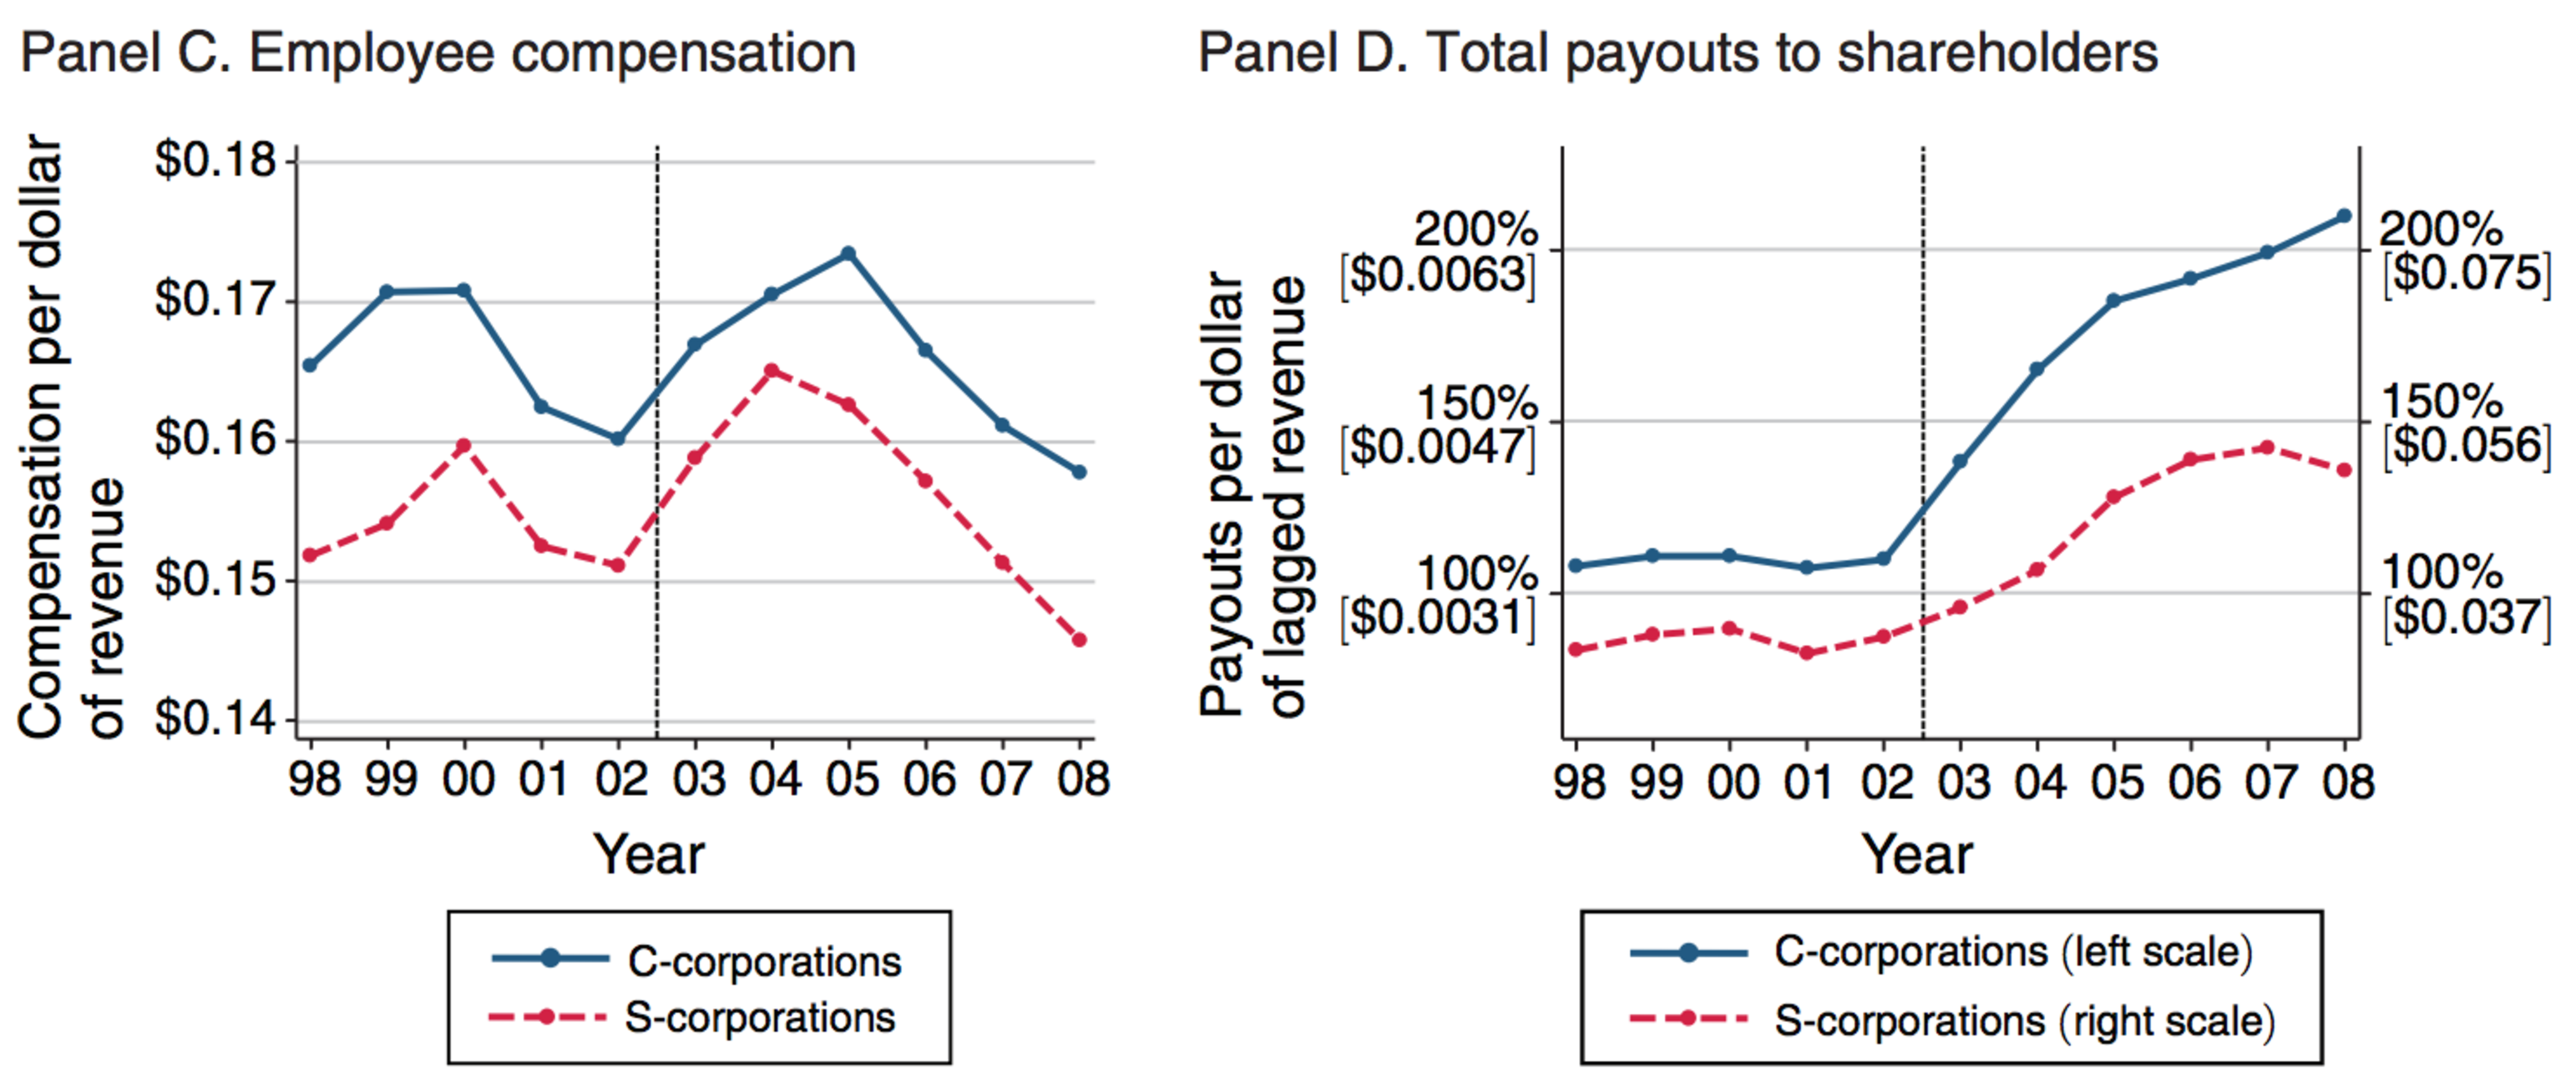
\includegraphics{images/yagan_2.pdf}
      }
      }
\end{frame}

\begin{frame}{Key Takeaway + threats}
  \begin{wideitemize}
  \item Tax reform had zero impact on differential investment and employee compensation
  \item Challenges orthodoxy on estimates of cost-of-capital elasticity of investment
  \item What are underlying challenges to identification?
    \begin{enumerate}
    \item Have to assume (and try to prove) that the only differential
      effect to S- vs C-corporations was through dividend tax changes
    \item During 2003, could other shocks differentially impact?
      \begin{itemize}
      \item Yes, accelerated depreciation -- but Yagan shows it
        impacts them similarly.
      \end{itemize}
    \end{enumerate}
  \item Key point: you have to make \emph{more} assumptions to assume
    that zero \textbf{differential} effect on investment implies zero
    \textbf{aggregate} effect.
  \end{wideitemize}
\end{frame}

\begin{frame}{Berger, Turner and Zwick (2019)}
  \begin{wideitemize}
  \item This paper studies the impact of temporary fiscal stimulus
    (First-Time Home Buyer tax credit) on housing markets
  \item Policy was differentially targetted towards first time home buyers
    \begin{itemize}
    \item Define program exposure as ``the number of potential
      first-time homebuyers in a ZIP code, proxied by the share of
      people in that ZIP in the year 2000 who are first-time
      homebuyers''
    \item The design:
      \begin{quote}
        The key threat to this design is the possibility that
        time-varying, place-specific shocks are correlated with our
        exposure measure.
      \end{quote}
    \end{itemize}
  \item This measure is \textbf{not} binary -- we are just comparing
    areas with a low share vs. high share, effectively. However, we
    have a dose-response framework in mind -- as we increase the
    share, the effect size should grow.
  \end{wideitemize}
\end{frame}

\begin{frame}{First stage: Binary approximation}
      \makebox[\linewidth][c]{
      \resizebox{0.7\linewidth}{!}{
      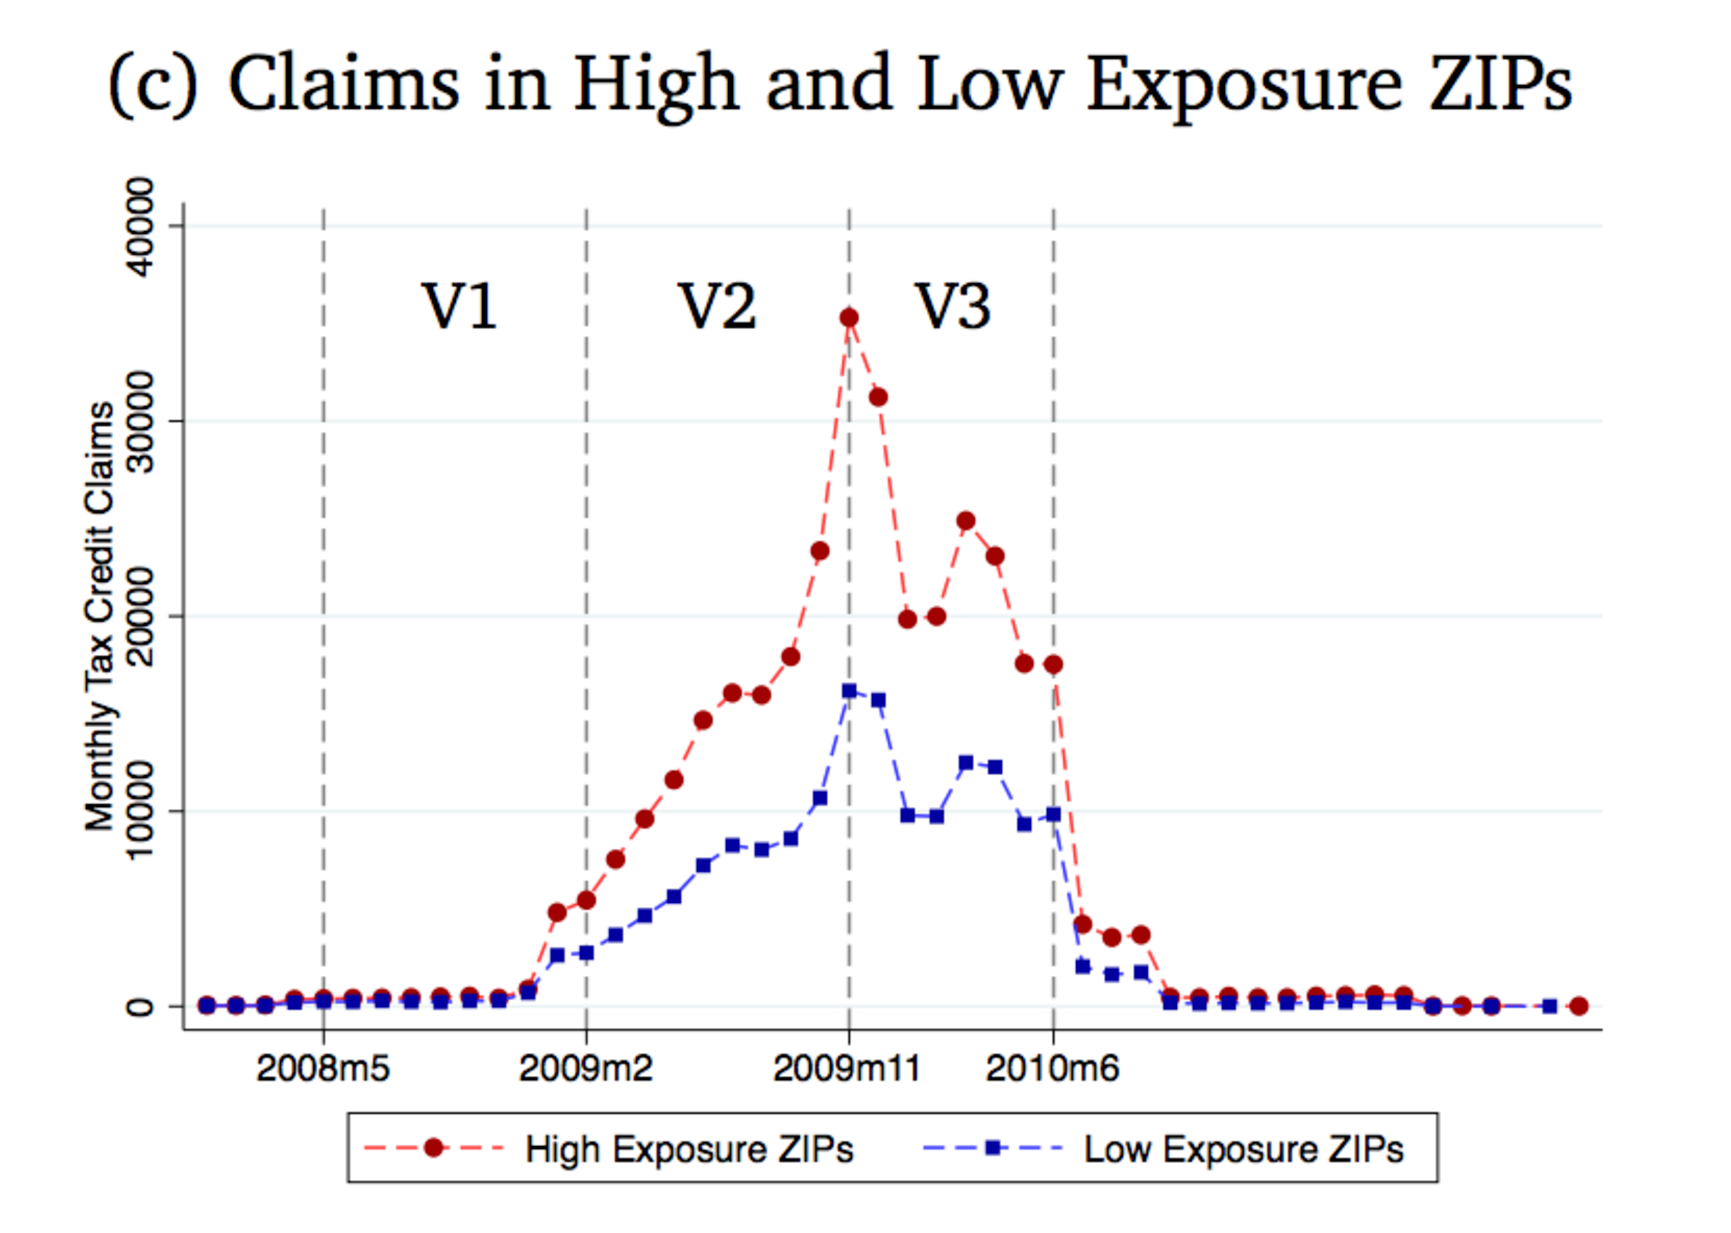
\includegraphics{images/zwick_fthb_1.pdf}
      }
      }
\end{frame}
\begin{frame}{First stage: Regression coefficients}
      \makebox[\linewidth][c]{
      \resizebox{0.7\linewidth}{!}{
      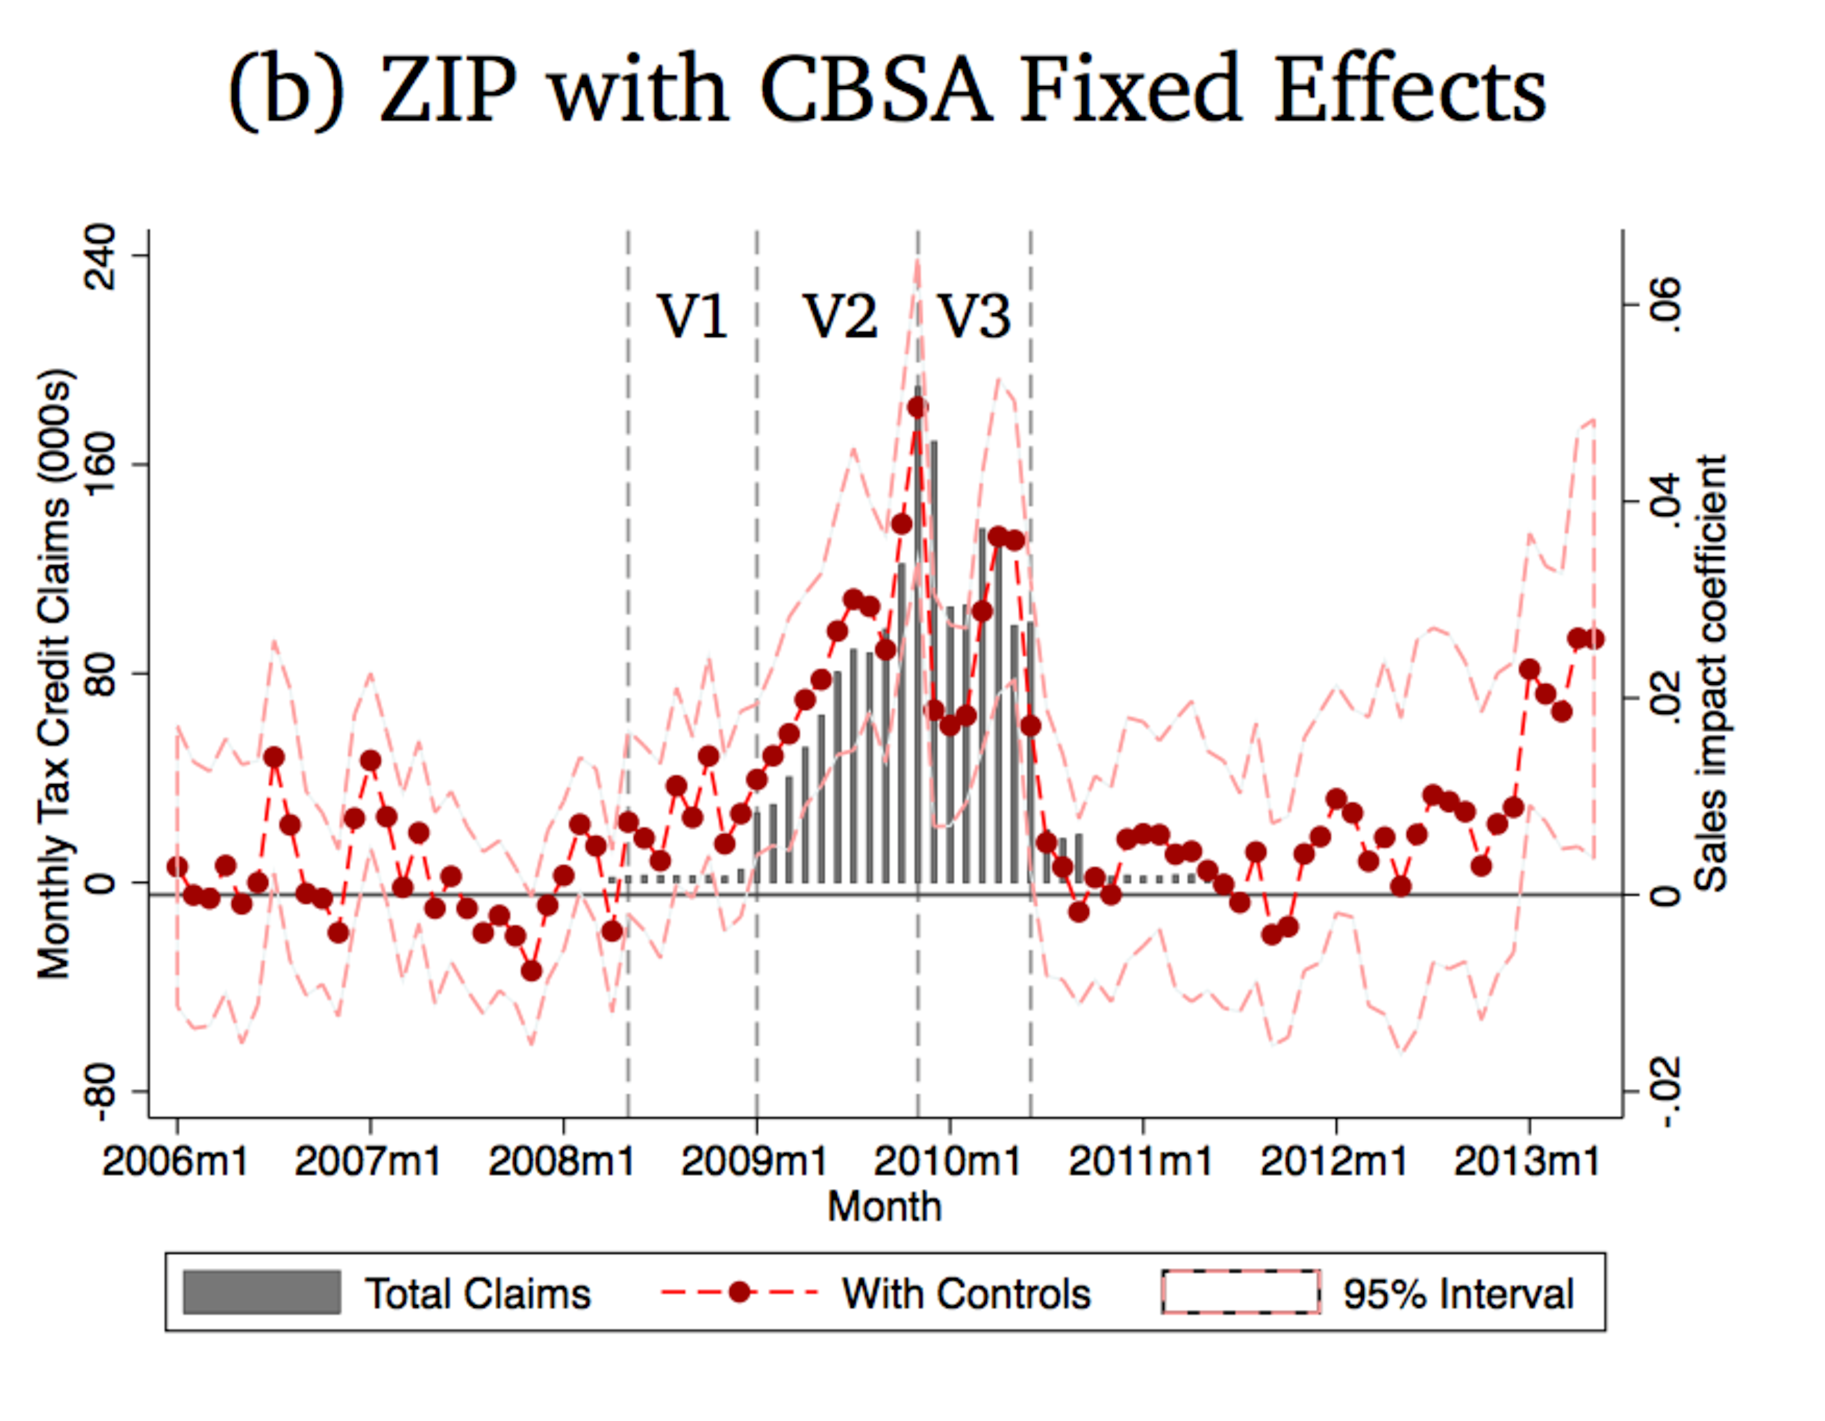
\includegraphics{images/zwick_fthb_2.pdf}
      }
      }
\end{frame}
\begin{frame}{Final Outcome: Regression coefficients}
      \makebox[\linewidth][c]{
      \resizebox{\linewidth}{!}{
      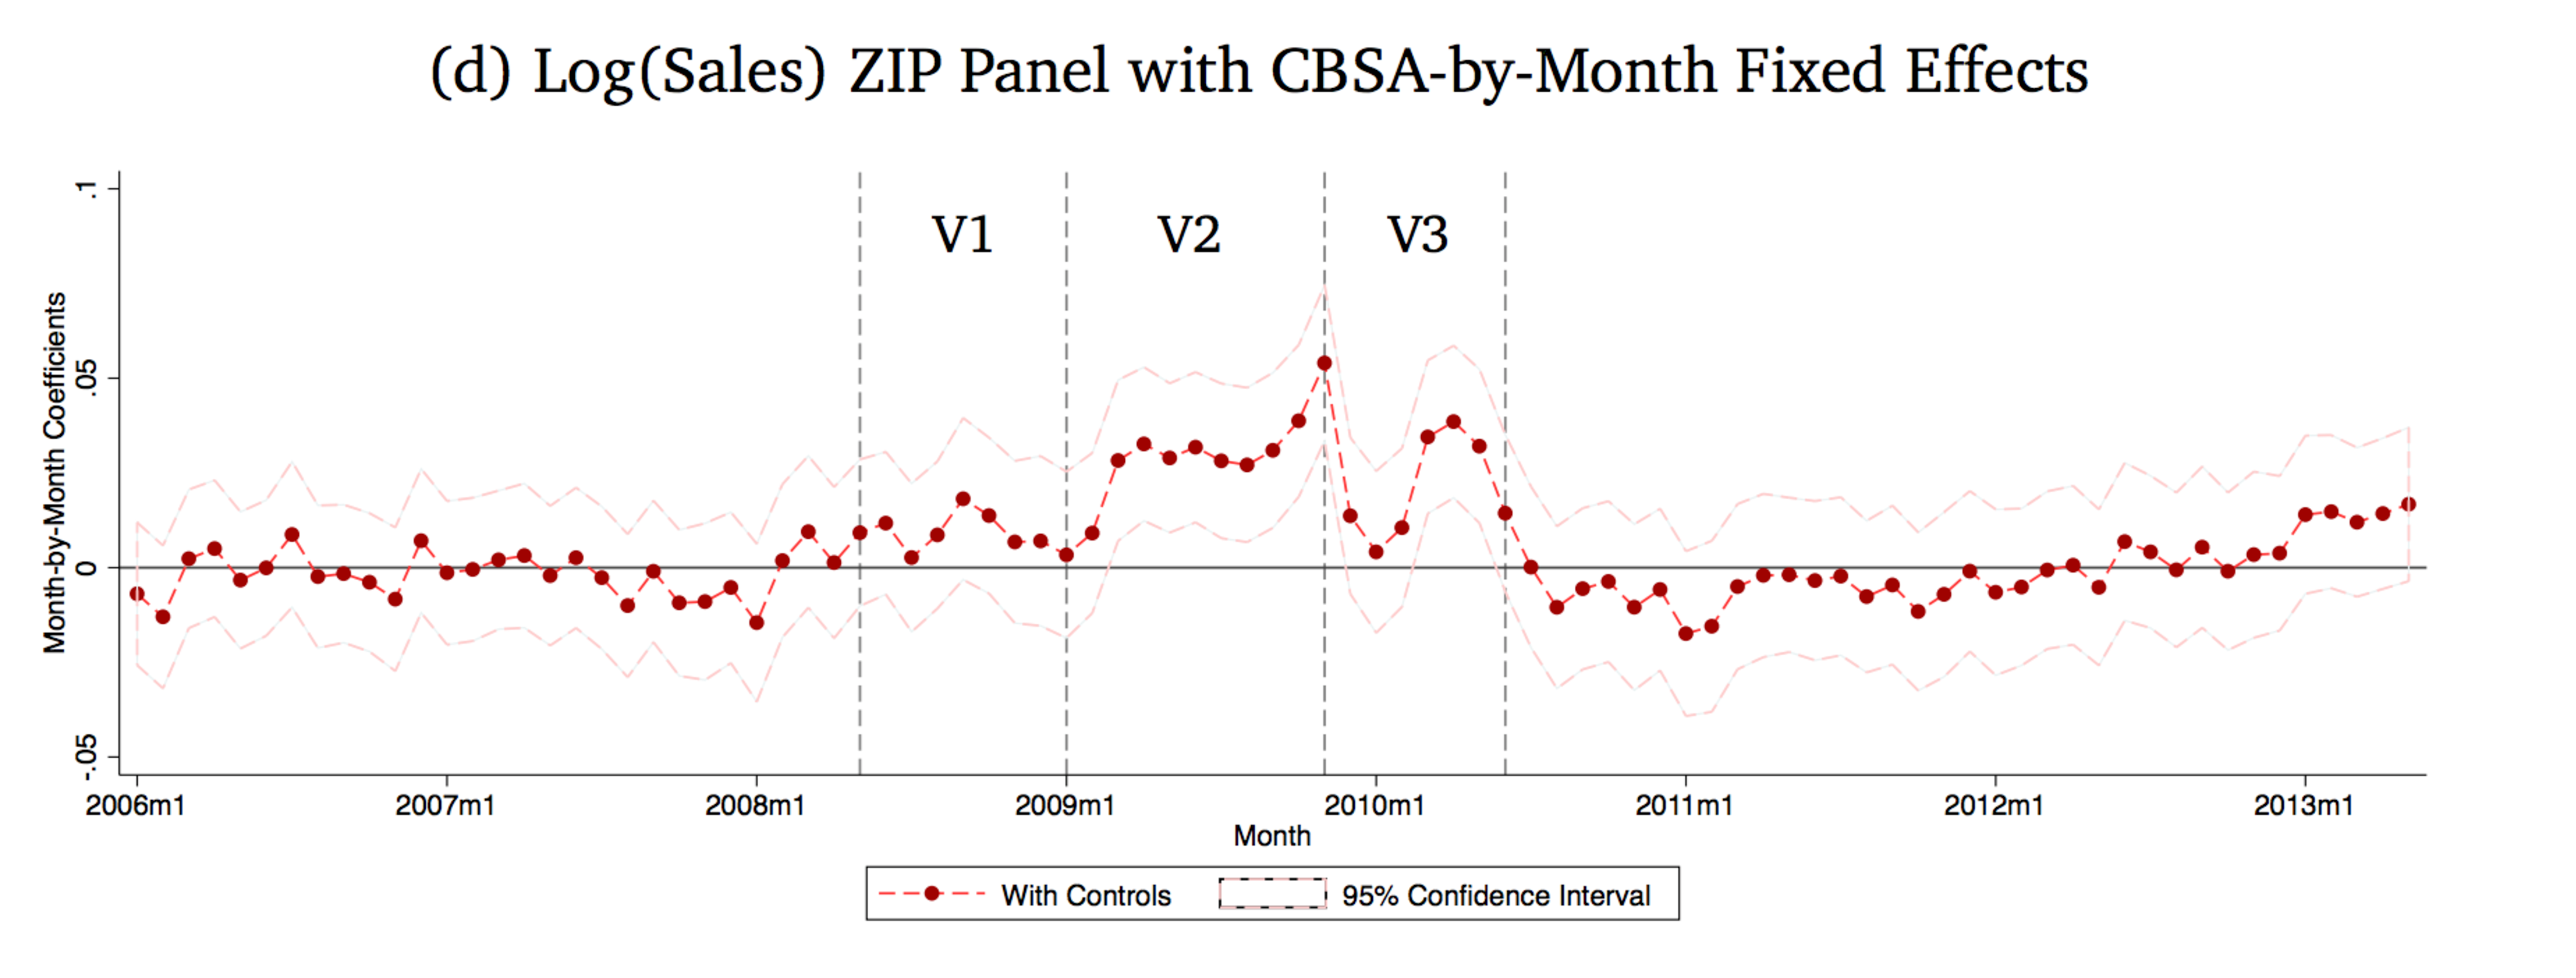
\includegraphics{images/zwick_fthb_3.pdf}
      }
      }
\end{frame}

\begin{frame}{Binary Approximation vs. Continuous Estimation}
  \begin{wideitemize}
    \item Remember our main equation did not necessarily specify that $D_{it}$ had to be binary. 
      \begin{equation}
      Y_{it} = \alpha_{i} + \gamma_{t} + \sum_{t=1, t\not=t_{0}}^{T}\delta_{t} D_{it} + \epsilon_{it},
    \end{equation}
  \item However, if it is continuous, we are making an additional
    strong functional form assumption that the effect of $D_{it}$ on our
    outcome is linear.
  \item We make this linear approximation all the time in our
    regression analysis, but it is worth keepping in mind. It is
    partially testable in a few ways:
    \begin{itemize}
    \item Bin the continuous $D_{it}$ into quartiles $\{\widetilde{D}_{itk}\}_{k=1}^{4}$ and estimate the effect across those groups:
      \begin{equation}
        Y_{it} = \alpha_{i} + \gamma_{t} + \sum_{t=1, t\not=t_{0}}^{T}\sum_{k=1}^{4}\delta_{t,k} \widetilde{D}_{it,k} + \epsilon_{it}.
      \end{equation}
    \item What does the ordering of $\delta_{t,k}$ look like? Is it at least monotonic?
    \end{itemize}
  \end{wideitemize}
\end{frame}

\begin{frame}{Berger, Turner and Zwick implementation of linearity test}
  \makebox[\linewidth][c]{
    \resizebox{0.7\linewidth}{!}{
      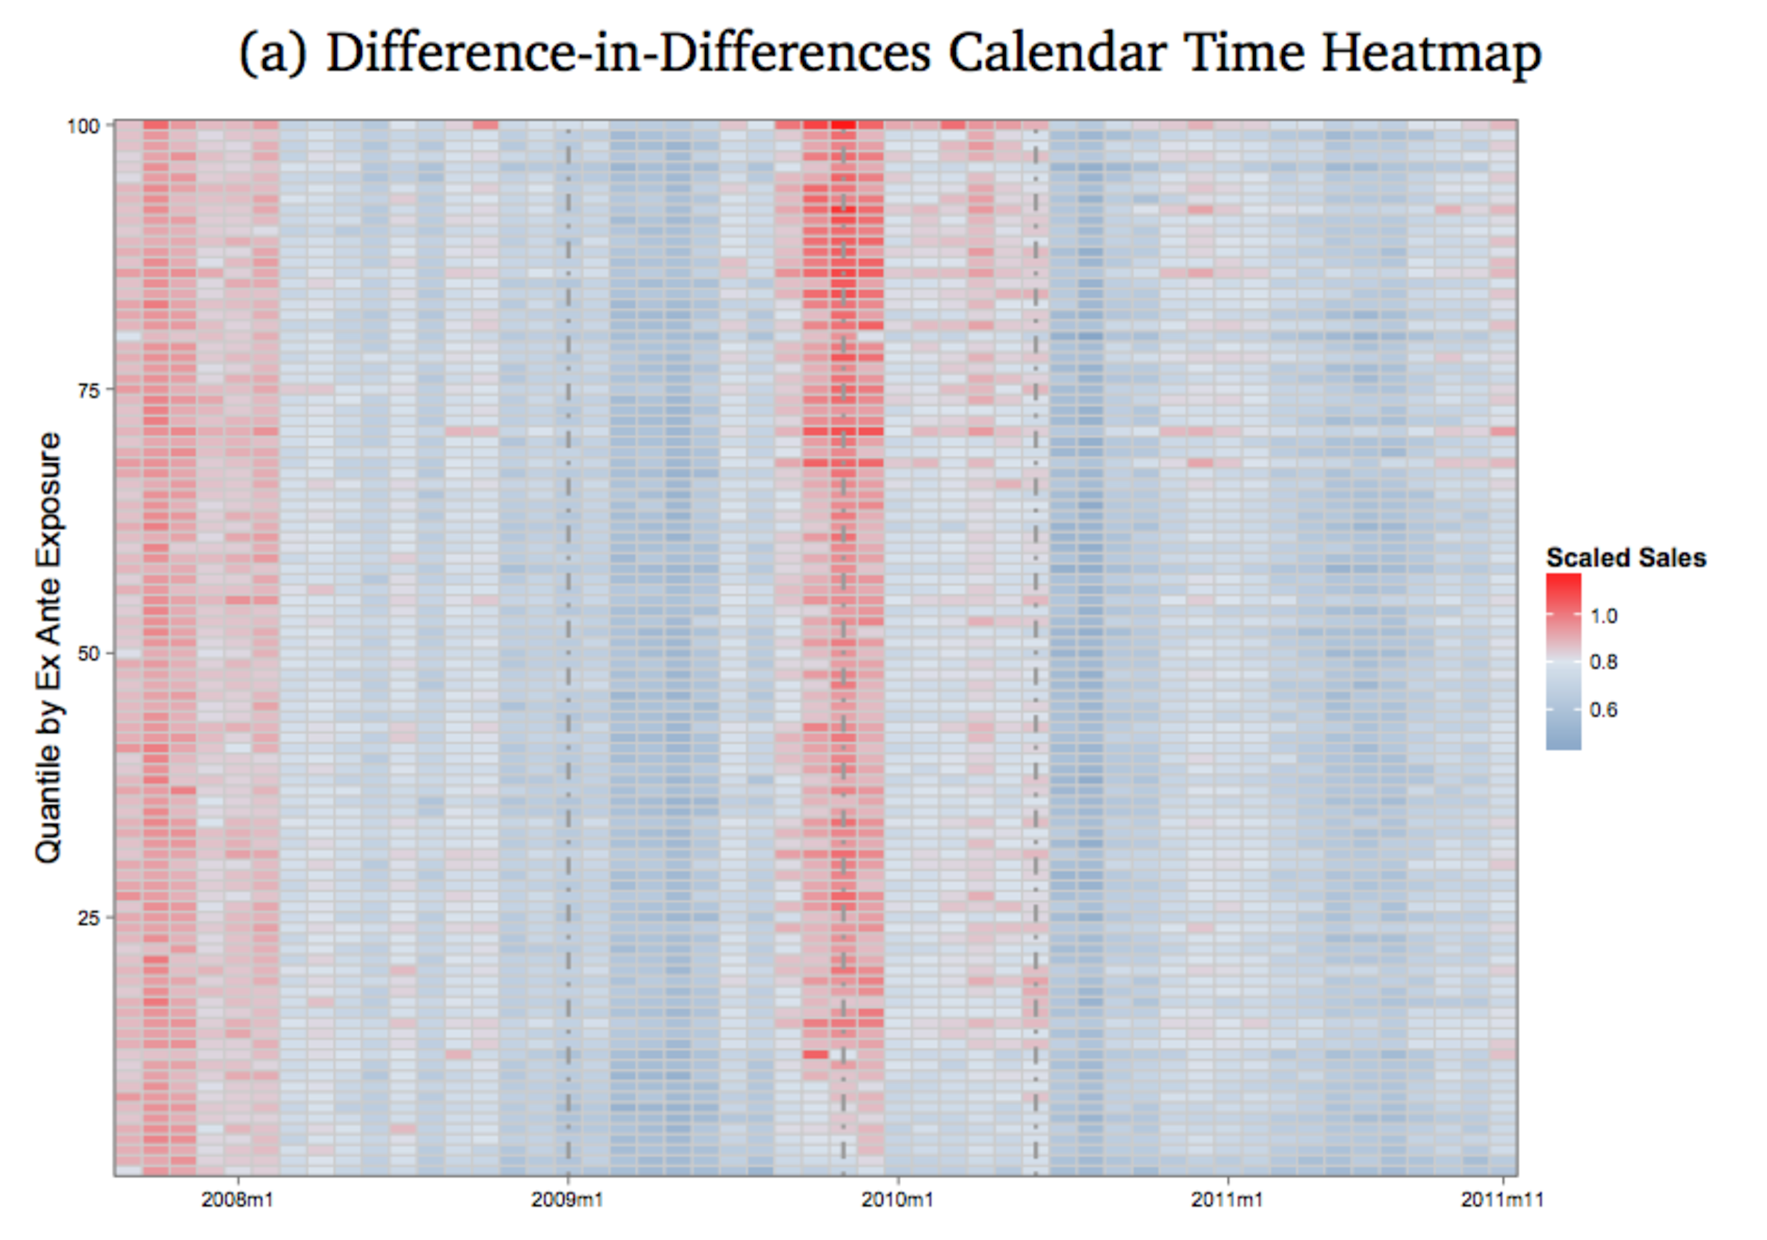
\includegraphics{images/zwick_fthb_4.pdf}
    }
  }
\end{frame}

\begin{frame}{Takeaway}
  \begin{wideitemize}
  \item When you have a continuous exposure measure, can be intuitive
    and useful to present binned means ``high'' and ``low'' groups
  \item However, best to present regression coefficients of the
    effects that exploits the full range of the continuous measure so
    that people don't think you're data mining
  \item Consider examining for non-monotonicities in your policy exposure measure
  \item This paper is still has only one ``shock'' -- one policy time period for implementation
  \end{wideitemize}
\end{frame}


\begin{frame}{Bailey and Goodman-Bacon (2015)}
  \begin{wideitemize}
  \item Paper studies  impact of rollout of Community Health Centers on mortality
    \begin{itemize}
    \item Idea is that CHCs can help lower mortality (esp. among
      elderly) by providing accessible preventative care
    \end{itemize}
  \item Exploit timing of implementation of CHCs
    \begin{quote}
        Our empirical strategy uses variation in when and where CHC
        programs were established to quantify their effects on
        mortality rates. The findings from two empirical tests support
        a key assumption of this approach—that the timing of CHC
        establishment is uncorrelated with other determinants of
        changes in mortality.
      \end{quote}
    \item Issue is that CHCs tend to be done in places
    \item Since CHCs are started in different places in different time
      periods, we estimate effects in \emph{event-time}, e.g. relative
      to initial rollout.
  \end{wideitemize}
\end{frame}

\begin{frame}{Negative effect on mortality}
    \makebox[\linewidth][c]{
    \resizebox{0.7\linewidth}{!}{
      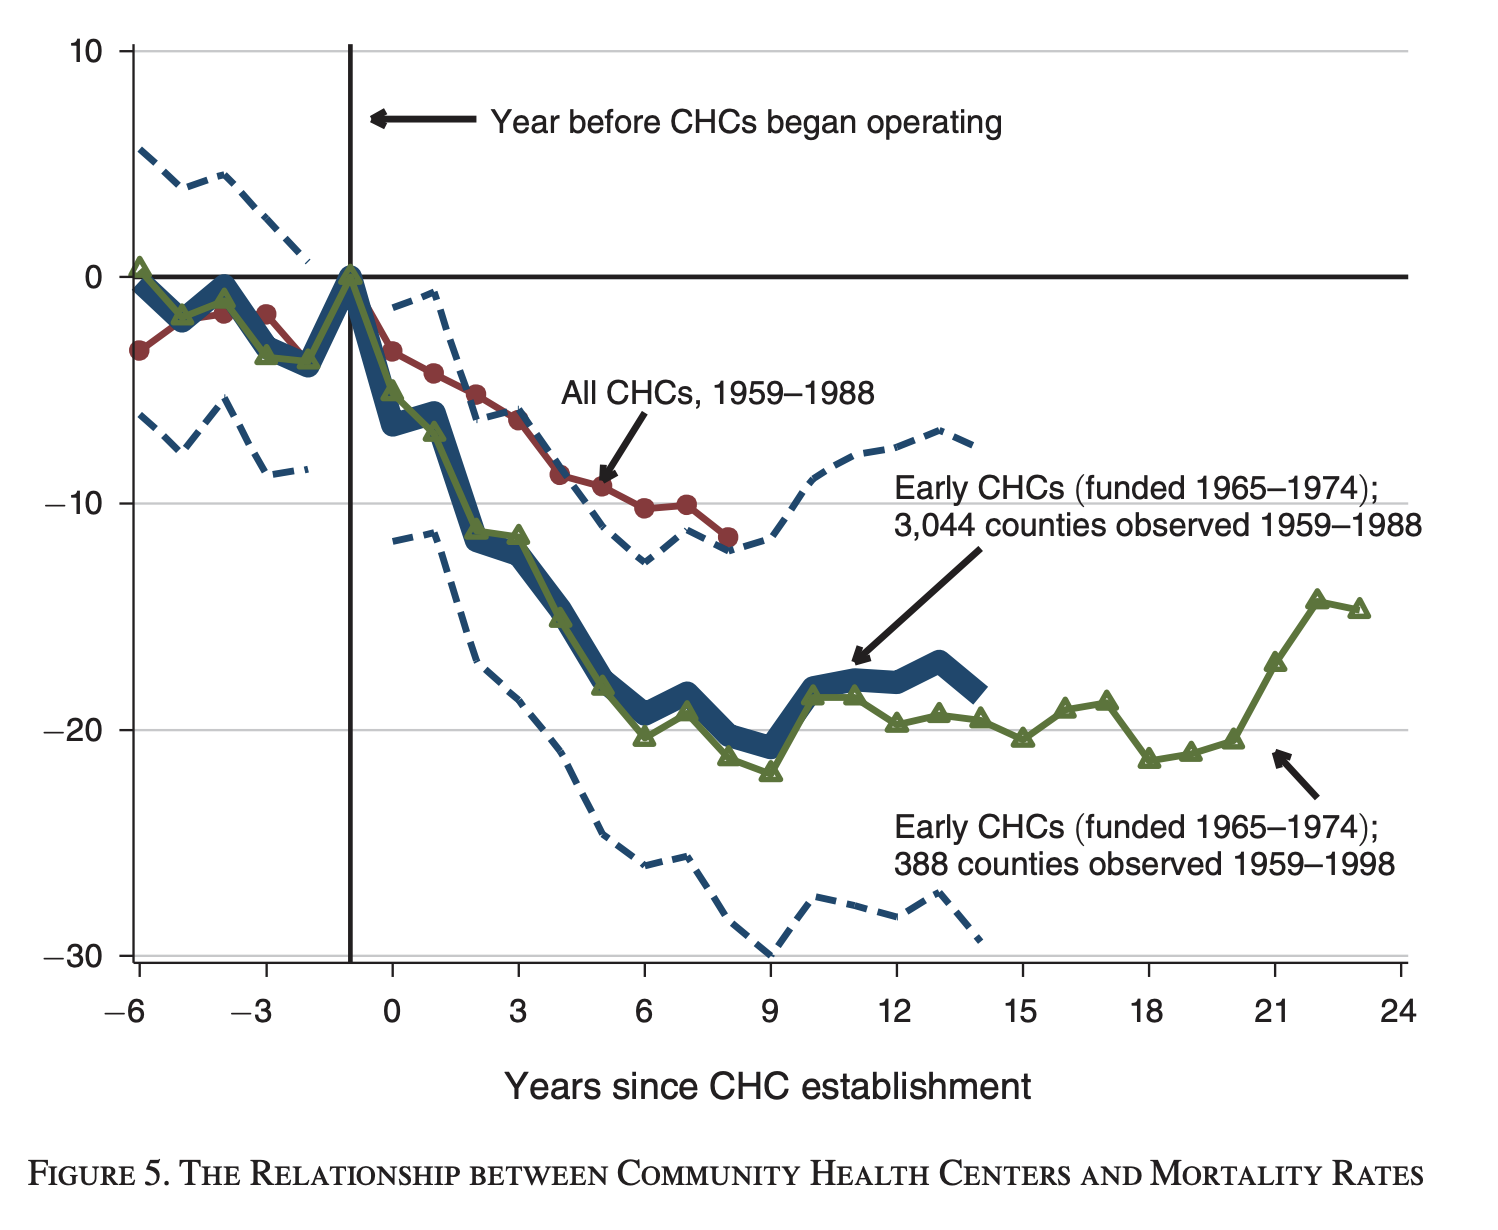
\includegraphics{images/baileygb.png}
    }
  }
\end{frame}
\begin{frame}{Negative effect on mortality, particularly among elderly}
    \makebox[\linewidth][c]{
    \resizebox{0.7\linewidth}{!}{
      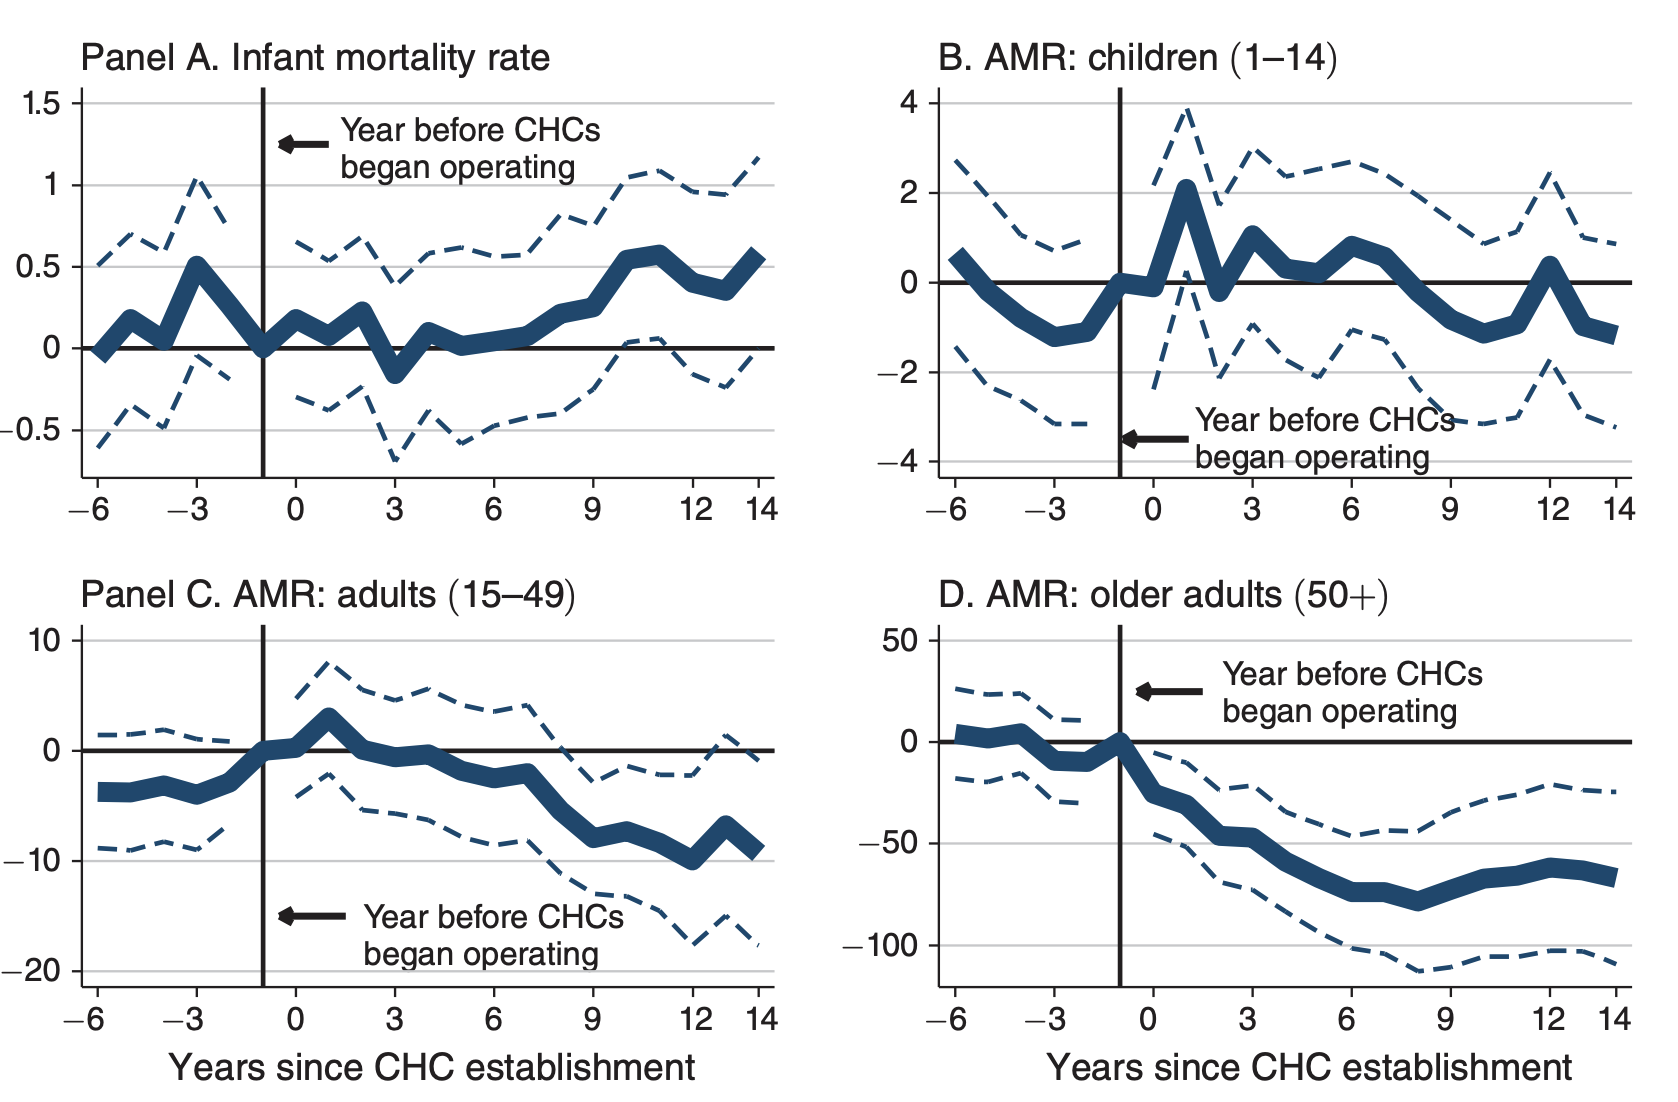
\includegraphics{images/baileygb2.png}
    }
  }
\end{frame}

\begin{frame}{Key takeaways}
  \begin{wideitemize}

    %%% ADD PIECE SHOWING WHY THERE"S POTENTIALLY A PROBLEM WITH ONLY ONE TIME PERIOD
    %%% ADD NOTATION WITH STAGGERED IMPLEMENTATION HERE
  \item Since the policy changes are staggered, we are less worried about effect driven by one confounding macro shock.
  \item Easier to defend story that has effects across different timings
    \begin{itemize}
    \item Also allows us to test for heterogeneity in the time series
    \end{itemize}
  \item Still makes the exact same identifying assumptions -- parallel
    trends in absence of changes
  \end{wideitemize}
\end{frame}



\begin{frame}{But a big issue emerges when we exploit differential timing}
  \begin{wideitemize}
  \item We have been extrapolating from the simple pre-post,
    treatment-control setting to broader cases
    \begin{itemize}
    \item multiple time periods of treatment
    \end{itemize}
  \item In fact, in some applications, the policy eventually hits everyone --
    we are just exploiting differential timing.
  \item If we run the ``two-way fixed effects'' model for these times of DinD
    \begin{equation}
      y_{it} = \alpha_{i} + \alpha_{t} + \beta^{DD}D_{it} + \epsilon_{it}
    \end{equation}
    what comparisons are we doing once we have lots of timings?
  \item Key point: is our \emph{estimator} mapping to our \emph{estimand}?
  \item Well, what's our estimand?
\end{wideitemize}
\end{frame}


\begin{frame}{What is our estimand with staggered timings?} 
  \begin{wideitemize}
  \item There are a huge host of papers touching on this question
  \item Callaway and Sant'anna (2020) propose the following building block estimand:
    \begin{equation}
      \tau_{ATT}(g,t) = E(Y_{it}(1) - Y_{it}(0) | D_{it} = 1 \forall t \geq g), 
    \end{equation}
    the ATT in period $t$ for those units whose treatment turns on in period $g$.
    \begin{itemize}
    \item In the 2x2 case, this was exactly our effect!
    \item This paper assumes absorbing treatment, but can be weakened in
      other papers (de Chaisemartin and d'Haultfoeuille (2020) discuss
      this)
    \end{itemize}
  \item It seems very reasonable that for our overall estimand, we
    want some weighted combinated of these ATTs
  \item Callaway and Sant'anna (2020) highlight two ways to identify the above estimand:
    \begin{enumerate}
    \item Parallel trends of treatment group with a group that is ``never-treated'' 
    \item Parallel trends of treatment group with the group of the ``not yet treated''
    \end{enumerate}
  \item Using these estimands, C\&S provide a very natural set of
    potential ways to aggregate these estimands up
  \end{wideitemize}

\end{frame}

\begin{frame}{Wait what happened to TWFE?}
  \begin{wideitemize}
  \item It turns out that the logic of the TWFE does not naturally extend to differential timings
    \begin{itemize}
    \item Recall that from our discussion of linear regression, regression is great because it does a variance weighted approximation:
      \begin{equation*}
        \tau = \frac{E(\sigma^{2}_{D}(W_{i})\tau(W_{i}))}{E(\sigma^{2}_{D}(W_{i}))}, \qquad \sigma^{2}_{D}(W_{i}) = E((D_{i} - E(D_{i}|W_{i}))^{2} | W_{i})
      \end{equation*}
  \item It turns out that in the panel setting with staggered timings,
    these weights are not necessarily positive
  \end{itemize}
\item Key insight from several papers: with staggered timings +
    heterogeneous effects, the TWFE approach to DinD (both using a
    single pooled estimator, or using an event study) can put large
    negative weight on certain groups' estimands, and large positive
    weight on others
    \begin{itemize}
    \item Serious issue for interpretability
    \item Some example papers: Borusyak and Jaravel (2017), de
      Chaisemartin and D’Haultfœuille (2020), Goodman-Bacon (2019),
      Sun and Abraham (2020)
    \end{itemize}
  \item Key point: this is \emph{solveable}. Merely a construct of
    being overly casual with estimator definition
  \end{wideitemize}
\end{frame}

\begin{frame}{Goodman-Bacon 2x2 comparisons}
  \begin{columns}[T] % align columns
    \begin{column}{0.4\textwidth}
      \begin{wideitemize}
      \item  Consider two staggered treatements and a never-treated group
      \item What does the TWFE estimator estimate?
      \end{wideitemize}
    \end{column}%
    \hfill%
    \begin{column}{.6\textwidth}
      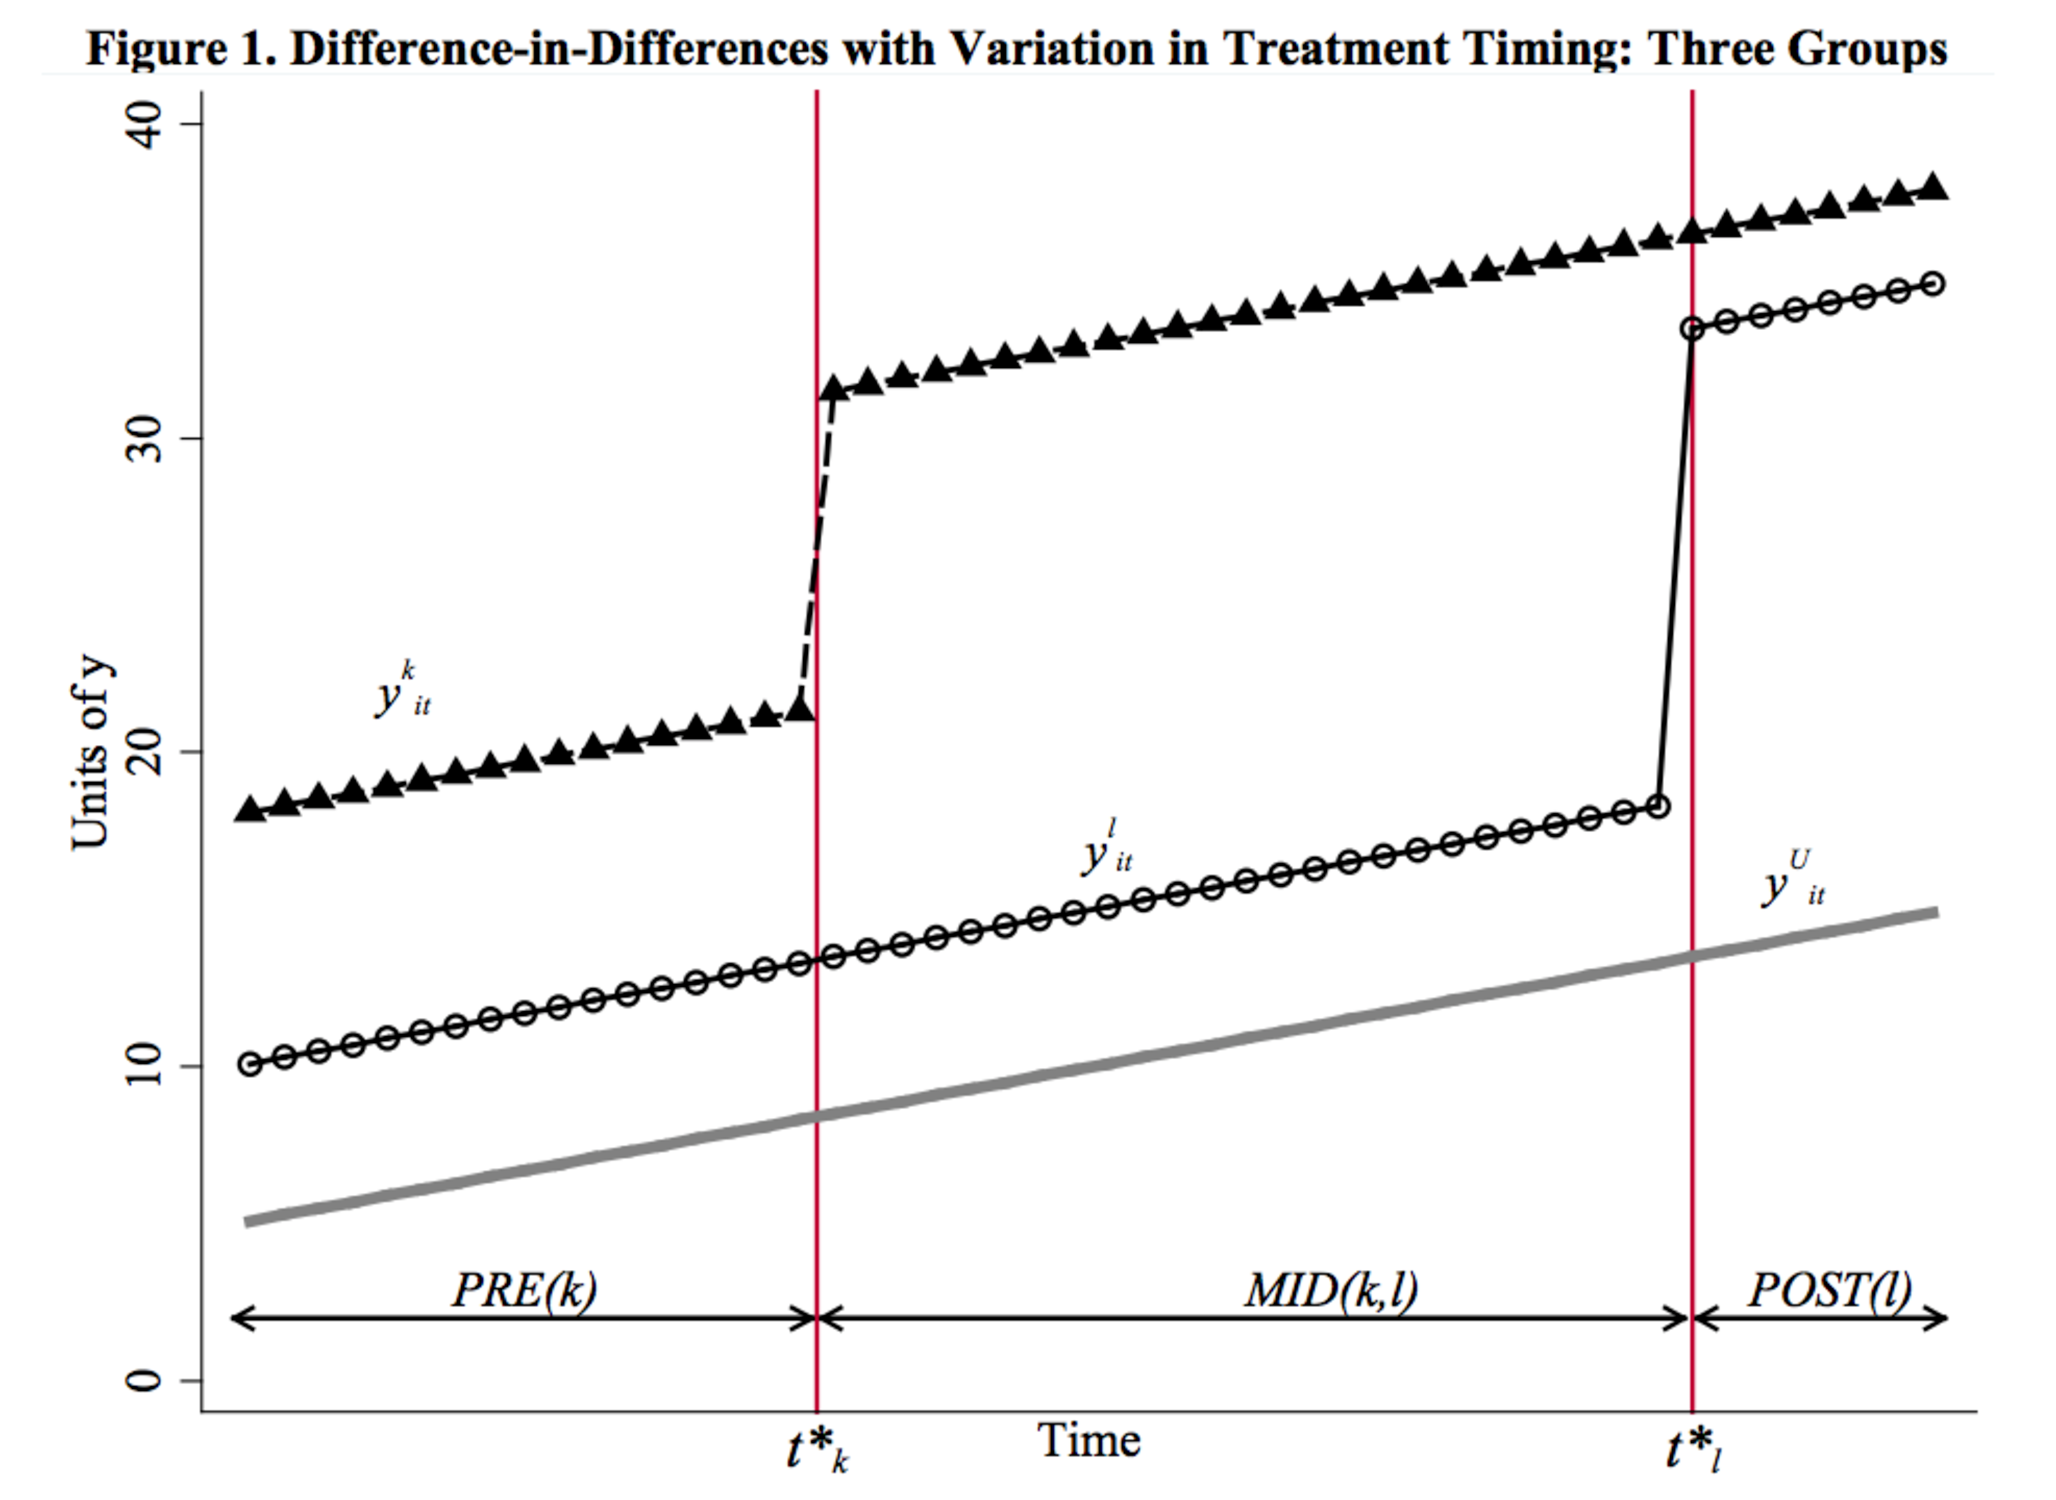
\includegraphics[width=\linewidth]{images/bacon_1.pdf}
    \end{column}%
  \end{columns}
\end{frame}
\begin{frame}{Goodman-Bacon 2x2 comparisons}
  \begin{columns}[T] % align columns
    \begin{column}{0.4\textwidth}
      \begin{wideitemize}
      \item Four potential comparisons that can be made
      \item turns out that TWFE DD estimator (pooled) is the 
        weighted average of all 2x2 comparisons
      \item These weights end up putting a high degree of weight on
        units treated in the middle of the sample (since they have the
        highest variance in the treatment indicator!)
      \end{wideitemize}
    \end{column}%
    \hfill%
    \begin{column}{.6\textwidth}
      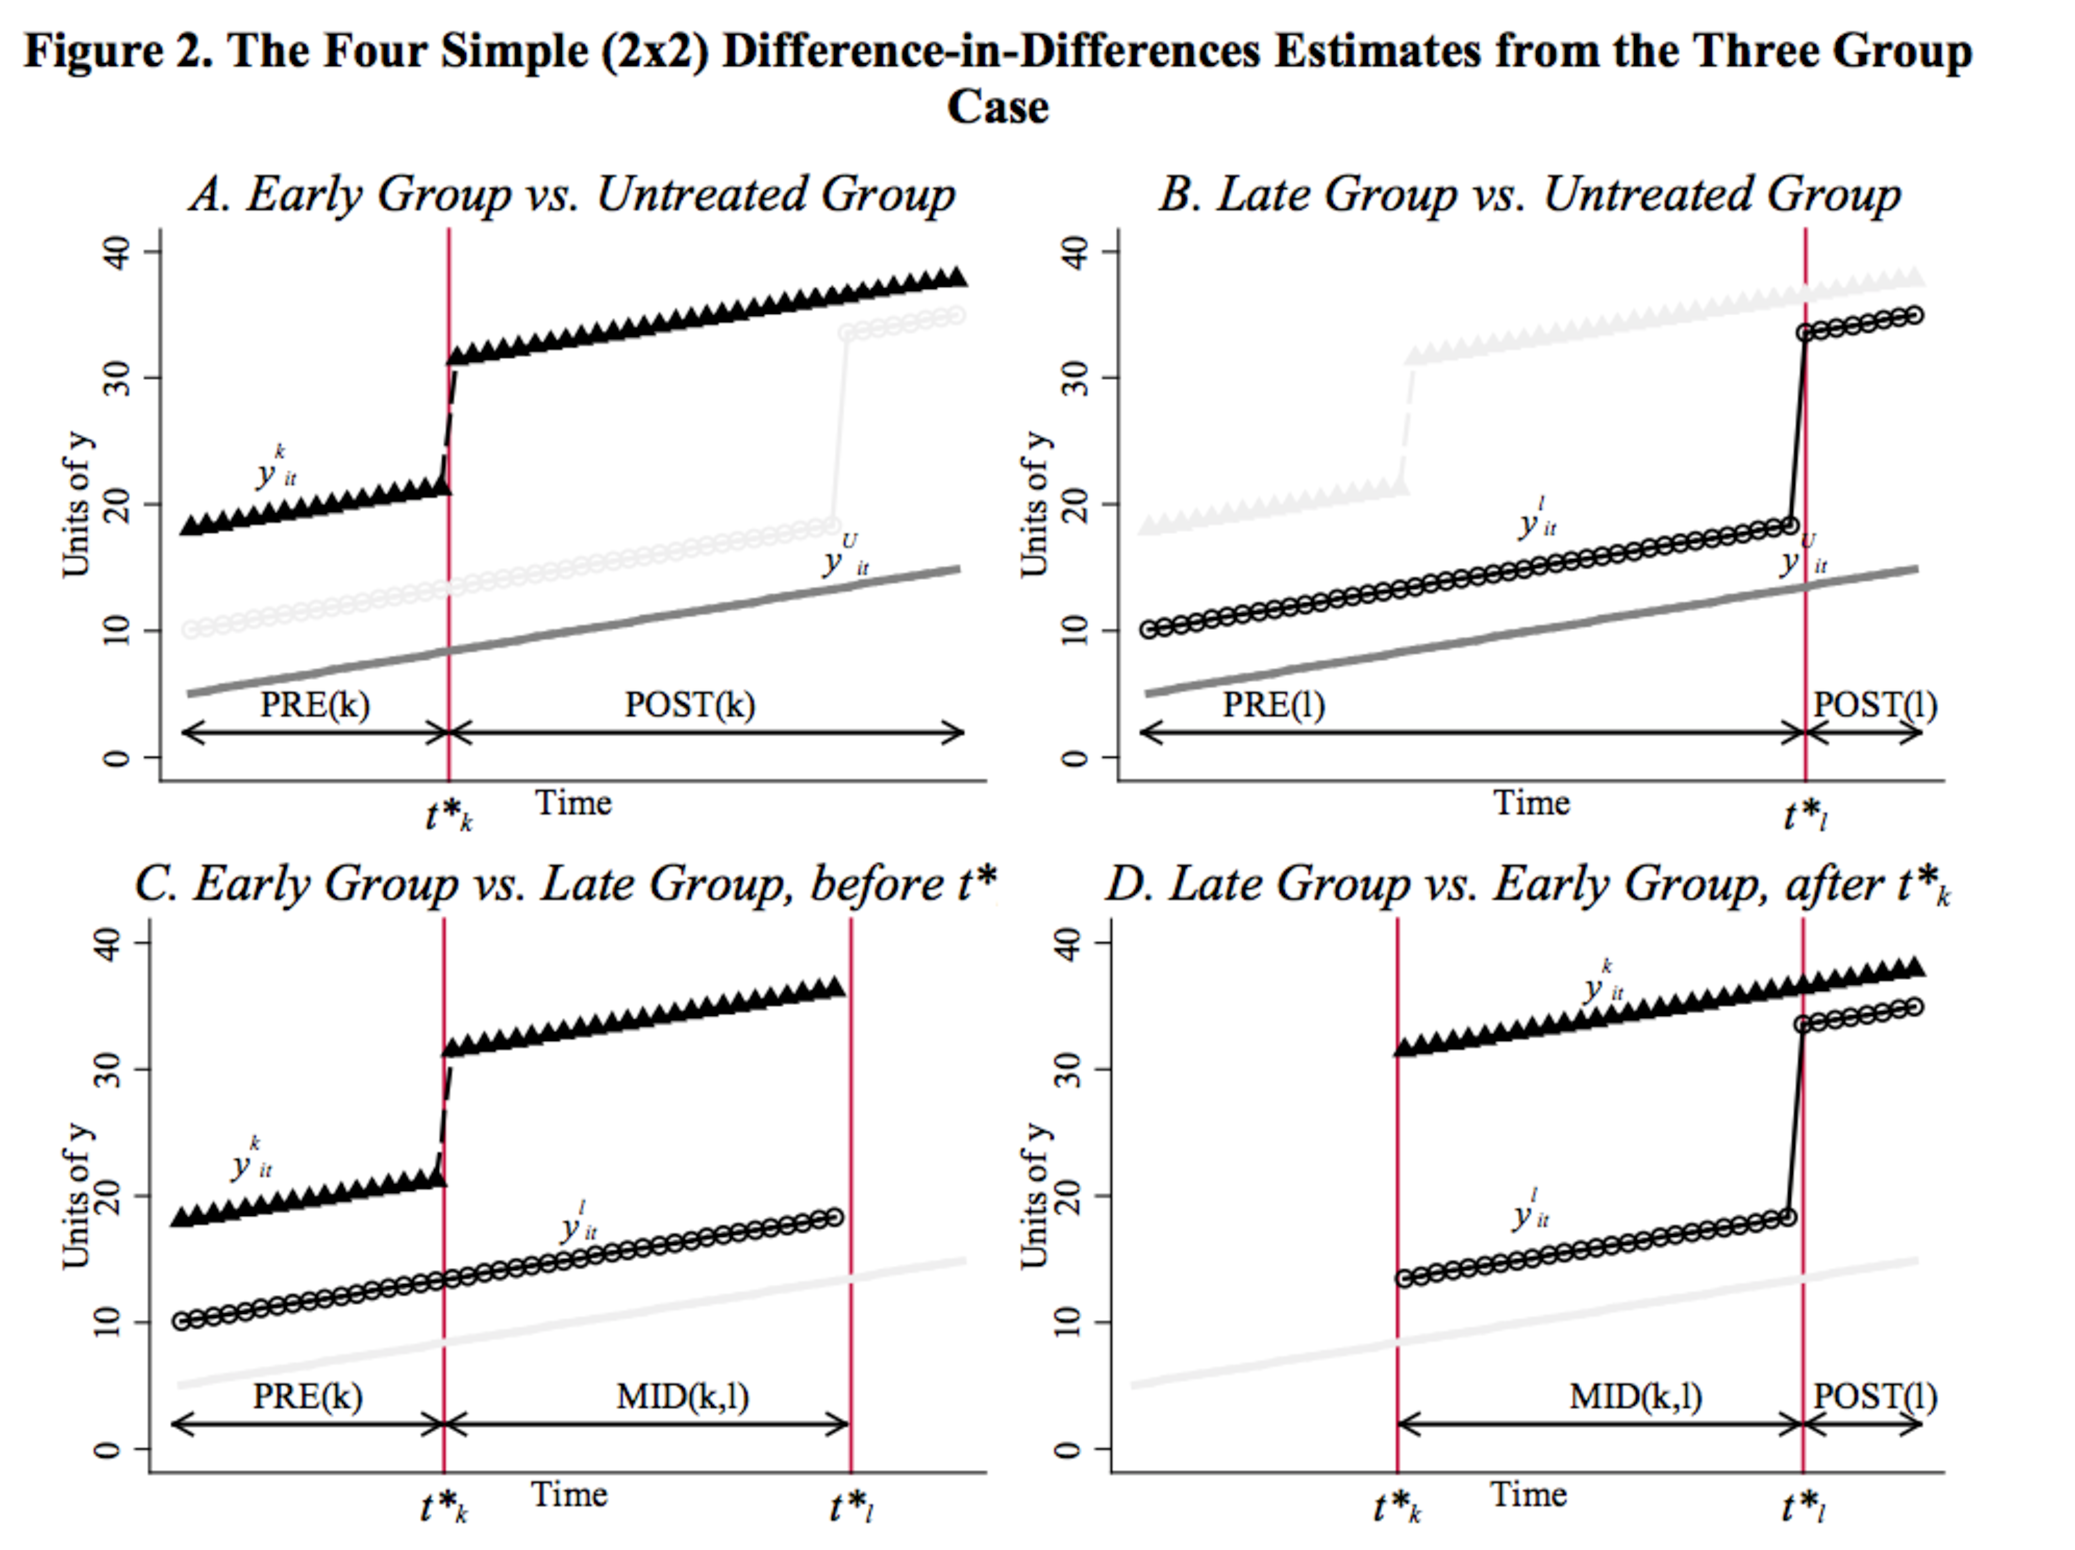
\includegraphics[width=\linewidth]{images/bacon_2.pdf}
    \end{column}%
  \end{columns}
\end{frame}

\begin{frame}{Goodman-Bacon 2x2 comparisons}
  \begin{columns}[T] % align columns
    \begin{column}{0.4\textwidth}
      \begin{wideitemize}
      \item<1-> The weighting becomes problematic if the effects vary
        over time -- if the effects are instantaneous and
        time-invariant, the weights are all positive
      \item<2-> However, time-varying effects create bad
        counterfactual groups, and create negative weights
      \item<2-> Goodman-Bacon provides a way to assess the weights in
        a given TWFE design
      \end{wideitemize}
    \end{column}%
    \hfill%
    \begin{column}{.6\textwidth}
      \only<1>{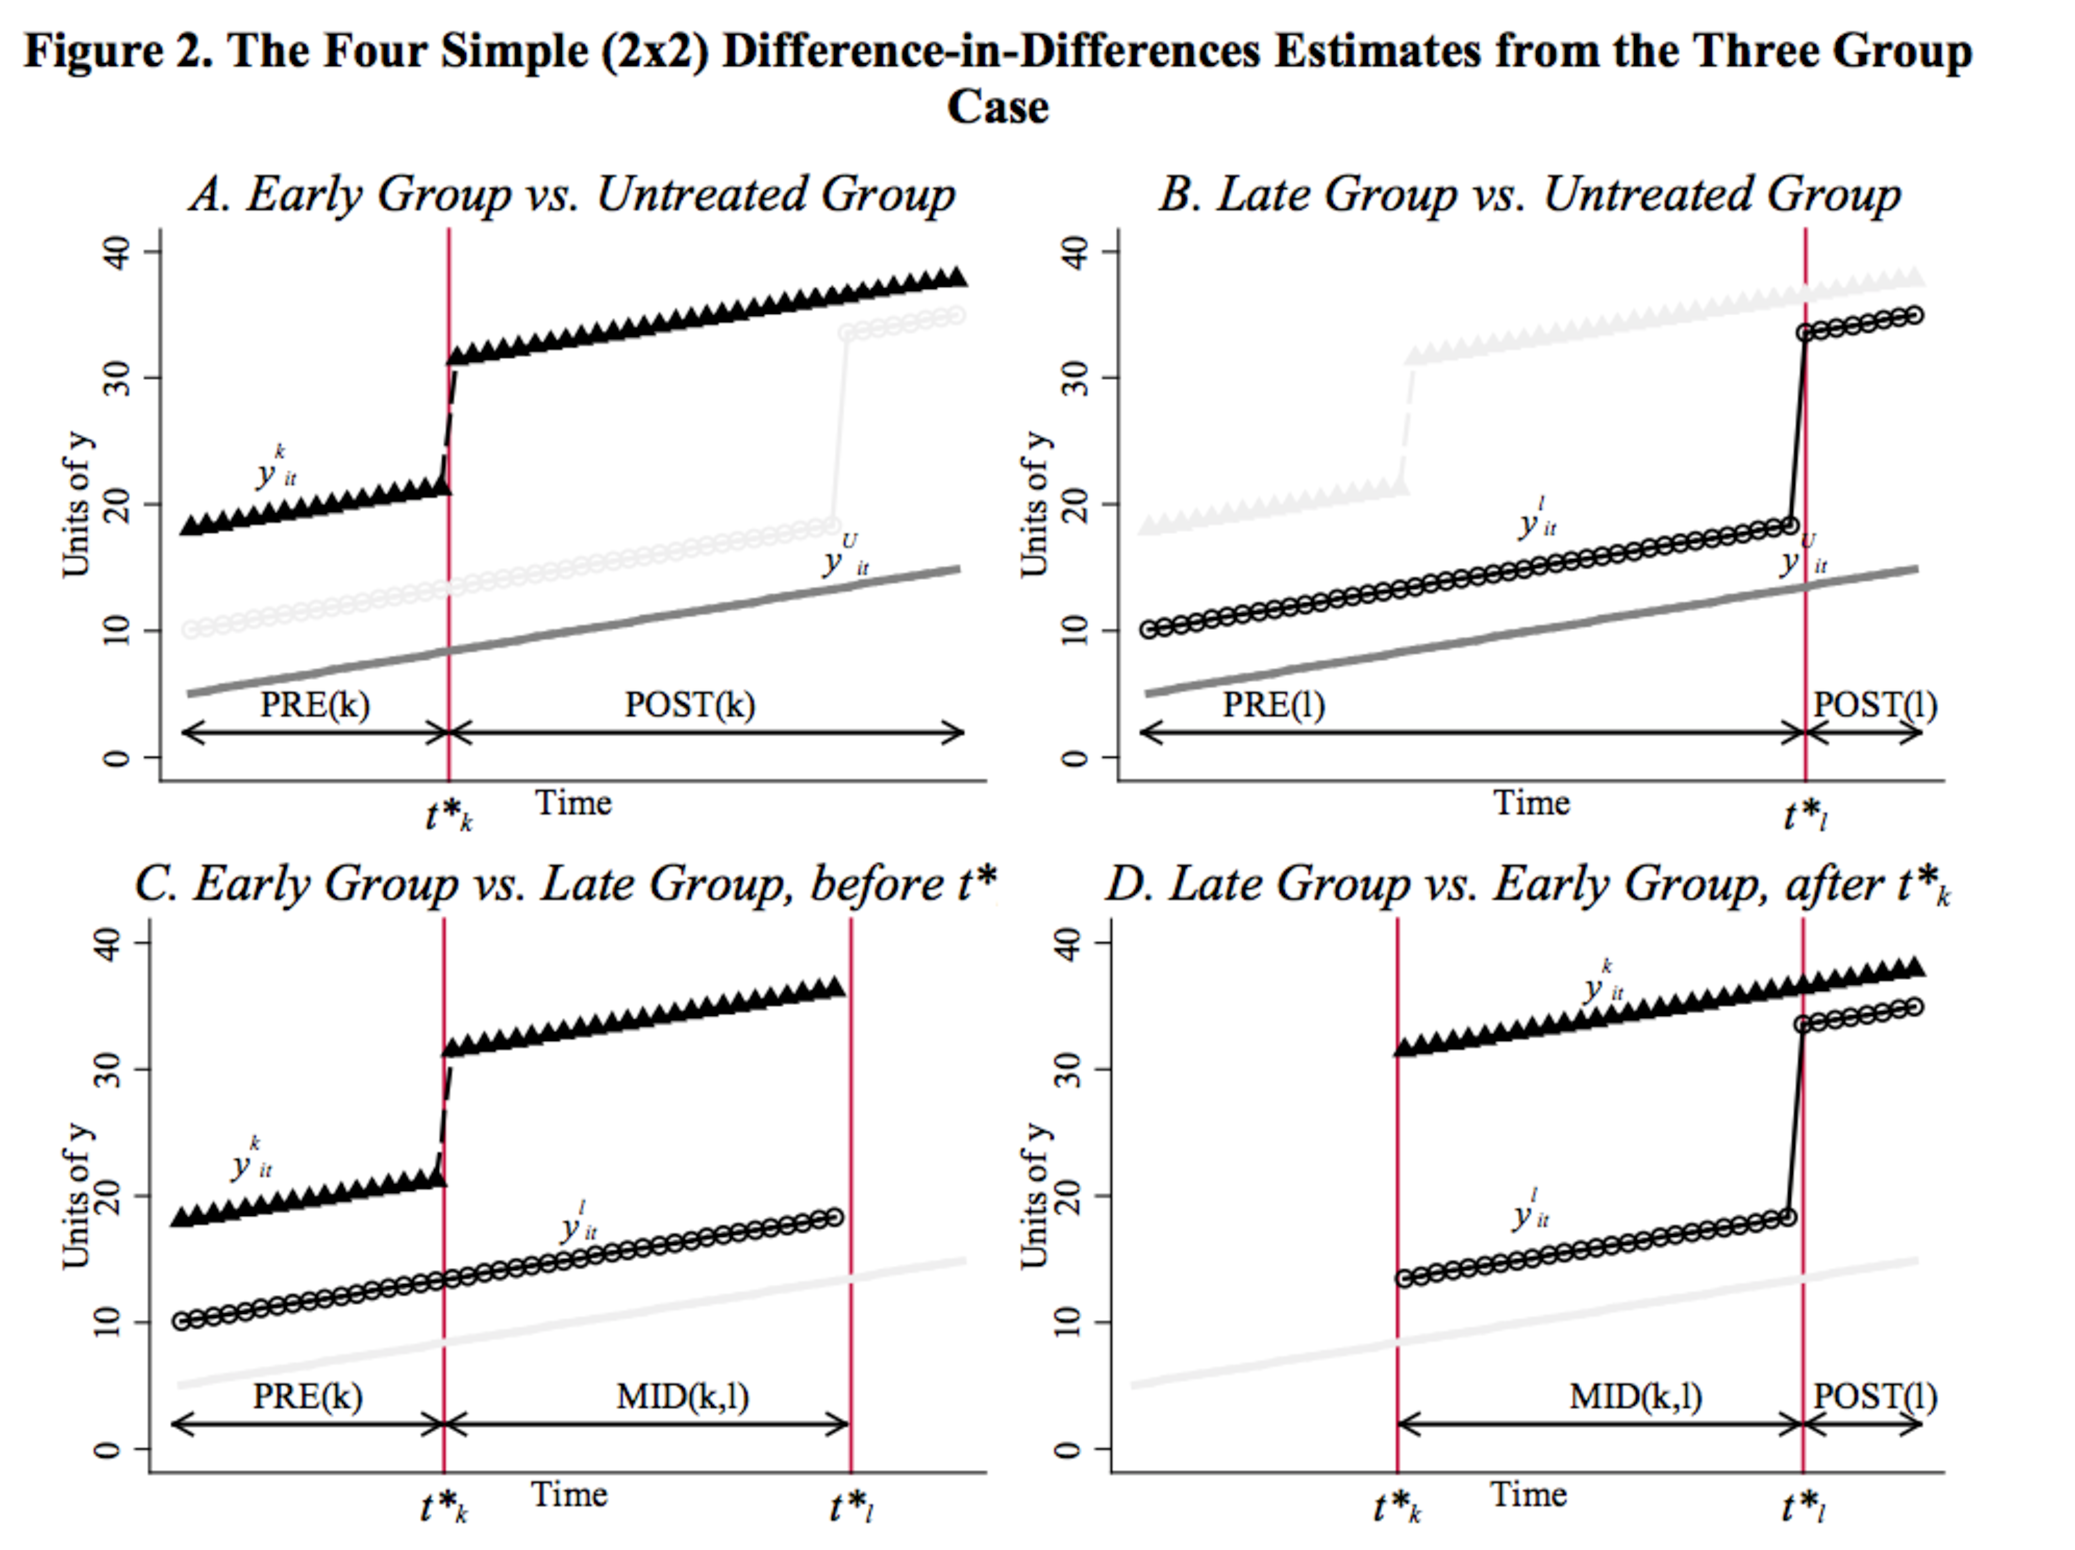
\includegraphics[width=\linewidth]{images/bacon_2.pdf}}
      \only<2>{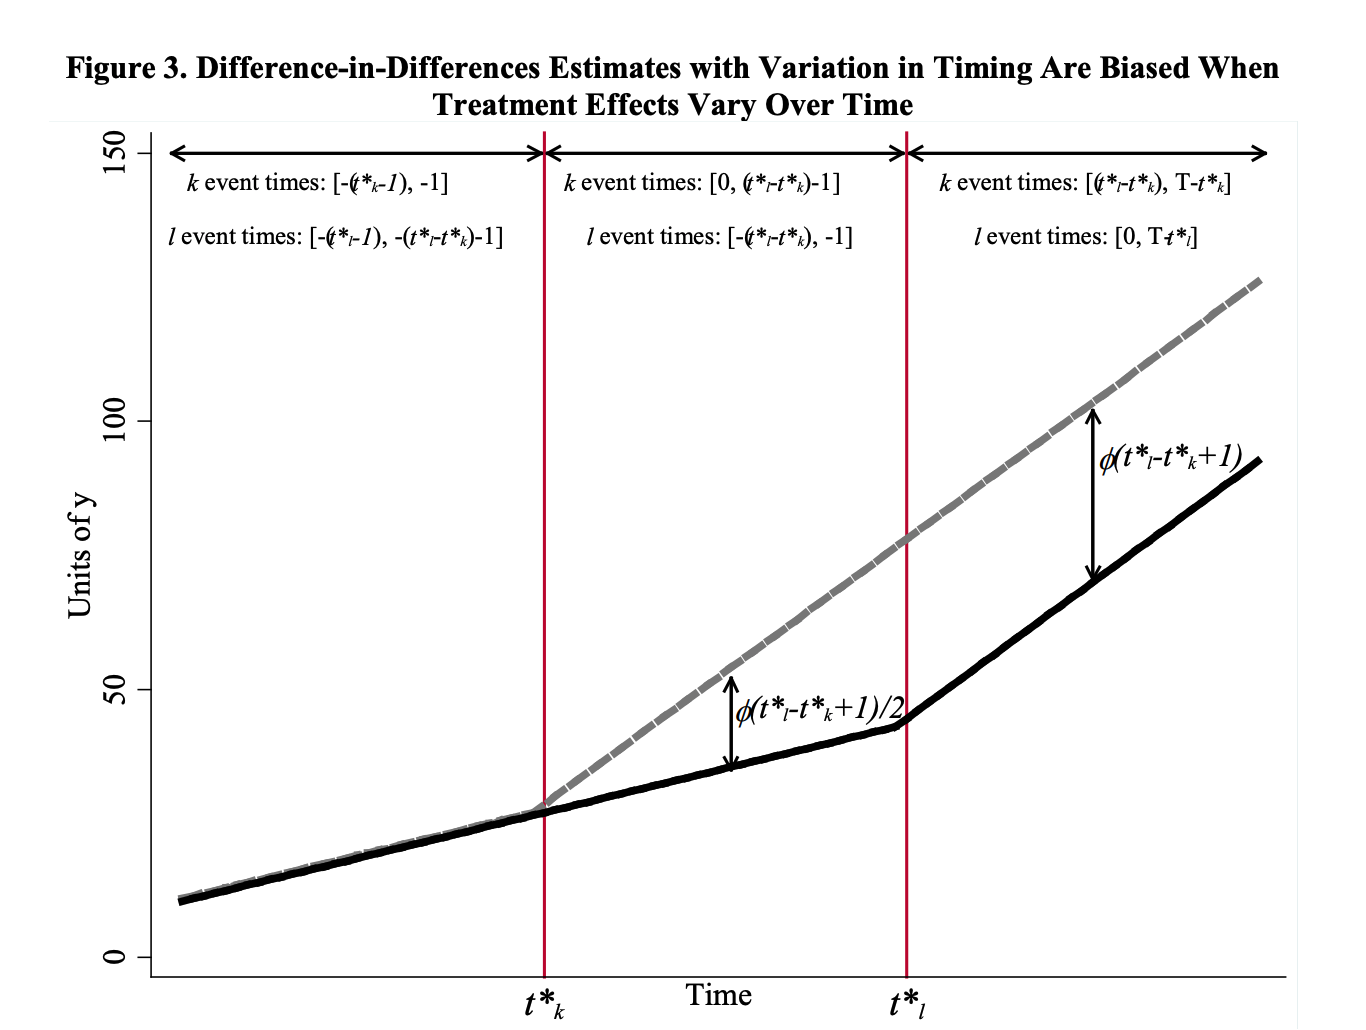
\includegraphics[width=\linewidth]{images/bacon_3.png}}      
    \end{column}%
  \end{columns}
\end{frame}


\begin{frame}{What to do with staggered timing in DinD?}
  \begin{wideitemize}
  \item There's really no reason to use the baseline TWFE in staggered timings
    \begin{itemize}
    \item A perfect example wherein the estimator does not generate an
      estimate that maps to a meaningful estimand
    \end{itemize}
  \item There are several approaches proposed in the literature that are just as good!
    \begin{itemize}
    \item Sun and Abraham (2020)
    \item de Chaisemartin and  d'Haultfoeuille (2020)
    \item Borusyak and Jaravel (2017)
    \item Callaway and Sant'anna (2020)      
    \end{itemize}
  \item These all are robust to this issue. I find Callaway and
    Sant'anna quite intuitive, but your circumstances may vary
    slightly. Key piece to keep in mind that differs a bit: 
    \begin{itemize}
    \item Is my treatment absorbing?
    \end{itemize}
  \item Irrespective of the exact paper, the key point is that we are
    generating a counterfactual and need to be careful that our
    estimator does so correctly
  \end{wideitemize}
\end{frame}


\begin{frame}{Finally, a discussion on inference}
  \begin{wideitemize}
  \item First, let's start with the old school fact that you must know
    if you are working with panel data and Dind
  \item \textbf{You must cluster on the unit of policy implementation
      if possible}. See Bertrand, Duflo and Mullainathan (2004)
    \begin{itemize}
    \item Why? Outcomes and the treatment tend to be severely
      autocorrelated within unit
    \item I say ``if possible'' since clearly in Card and Krueger that
      is infeasible
    \end{itemize}
  \item If the policy variation is implemented at the industry level,
    you should not cluster at the firm level
  \item If the policy variation is implemented at the firm level, you
    cannot use robust standard errors
  \end{wideitemize}
\end{frame}

\begin{frame}{Small clusters}
  \begin{wideitemize}
  \item The Card and Krueger case was too extreme, but there are approaches for dealing with a small number of clusters
  \item This approach typically involves  bootstrapping, and can handle small number of treated groups relative to the overall population
  \item See Andreas Hagemann's work for a place to start
  \end{wideitemize}
\end{frame}

\begin{frame}{Uniform confidence intervals}
  \begin{wideitemize}
  \item Finally, when considering event study graphs, pre-trend graphs
    should use uniform confidence intervals, rather than pointwise confidence intervals
    \begin{itemize}
    \item Advocated for by Freyaldenhoven et al (2018):
    \end{itemize}
  \item Code available here thanks to Ryan Kessler: \url{https://github.com/paulgp/simultaneous_confidence_bands}
    \begin{center}
    \only<1>{    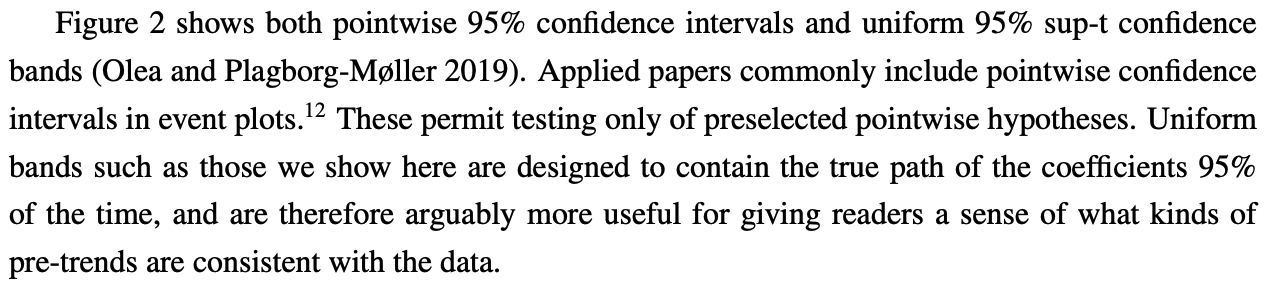
\includegraphics[width=\linewidth]{images/freyaldenhoven1.png}}
    \only<2>{    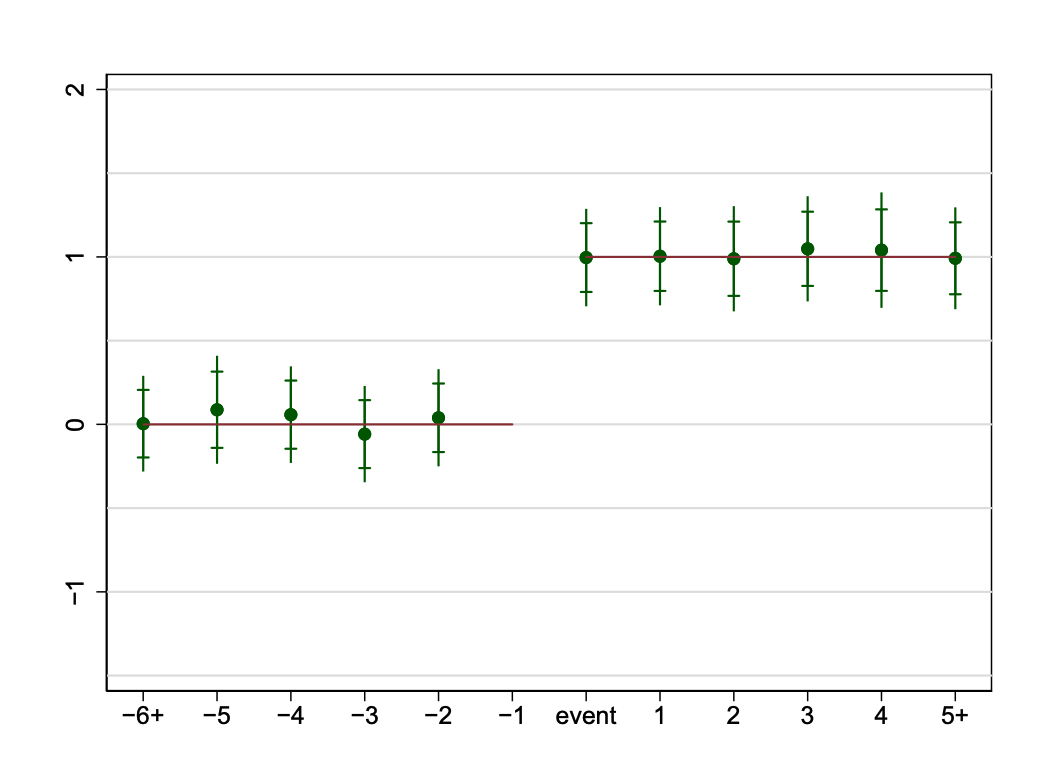
\includegraphics[width=0.5\linewidth]{images/freyaldenhoven2.png}}
    \end{center}
  \end{wideitemize}
\end{frame}


\begin{frame}{Conclusion}
  \begin{wideitemize}
  \item Difference in difference is hugely powerful in applied settings
  \item Does not require random assignment, but rather implementation
    of policies that differentially impacts different groups and is
    not confounded by other shocks at the same time.
  \item Can be a great application of big data, with convincing graphs
    that highlight your application
  \item Also allows for partial tests of identifying assumptions
  \item Worth carefully thinking about what your identifying
    assumptions are in each setting, and transparently highlighting
    them.
  \item Important to note that this always identifies a
    \emph{relative} affect, and to aggregate, you will typically need
    a model and additional strong assumptions (see Auclert, Dobbie and
    Goldsmith-Pinkham (2019) for an example in a macro setting).
  \end{wideitemize}
\end{frame}

\begin{frame}{My takeaways from new literature}
  \begin{wideitemize}
  \item Beware weak tests of pre-trends. Consider using R\&R's
    partial identification tests to assess robustness of results. 
  \item Do not worry about the new literature on staggered timings if you only have one timing!
  \item Think carefully about your estimand if you're using a staggered timing DinD -- what's your counterfactual in each case?
    \begin{itemize}
    \item Software exists for many of these papers. This is doable!
    \end{itemize}
  \item When plotting confidence intervals in event studies, you should plot uniform confidence intervals.
  \end{wideitemize}
\end{frame}
\end{document}